% Options for packages loaded elsewhere
\PassOptionsToPackage{unicode}{hyperref}
\PassOptionsToPackage{hyphens}{url}
%
\documentclass[
]{book}
\usepackage{lmodern}
\usepackage{amssymb,amsmath}
\usepackage{ifxetex,ifluatex}
\ifnum 0\ifxetex 1\fi\ifluatex 1\fi=0 % if pdftex
  \usepackage[T1]{fontenc}
  \usepackage[utf8]{inputenc}
  \usepackage{textcomp} % provide euro and other symbols
\else % if luatex or xetex
  \usepackage{unicode-math}
  \defaultfontfeatures{Scale=MatchLowercase}
  \defaultfontfeatures[\rmfamily]{Ligatures=TeX,Scale=1}
\fi
% Use upquote if available, for straight quotes in verbatim environments
\IfFileExists{upquote.sty}{\usepackage{upquote}}{}
\IfFileExists{microtype.sty}{% use microtype if available
  \usepackage[]{microtype}
  \UseMicrotypeSet[protrusion]{basicmath} % disable protrusion for tt fonts
}{}
\makeatletter
\@ifundefined{KOMAClassName}{% if non-KOMA class
  \IfFileExists{parskip.sty}{%
    \usepackage{parskip}
  }{% else
    \setlength{\parindent}{0pt}
    \setlength{\parskip}{6pt plus 2pt minus 1pt}}
}{% if KOMA class
  \KOMAoptions{parskip=half}}
\makeatother
\usepackage{xcolor}
\IfFileExists{xurl.sty}{\usepackage{xurl}}{} % add URL line breaks if available
\IfFileExists{bookmark.sty}{\usepackage{bookmark}}{\usepackage{hyperref}}
\hypersetup{
  pdftitle={Quantifying Life},
  pdfauthor={Dmitry Kondrashov},
  hidelinks,
  pdfcreator={LaTeX via pandoc}}
\urlstyle{same} % disable monospaced font for URLs
\usepackage{color}
\usepackage{fancyvrb}
\newcommand{\VerbBar}{|}
\newcommand{\VERB}{\Verb[commandchars=\\\{\}]}
\DefineVerbatimEnvironment{Highlighting}{Verbatim}{commandchars=\\\{\}}
% Add ',fontsize=\small' for more characters per line
\usepackage{framed}
\definecolor{shadecolor}{RGB}{248,248,248}
\newenvironment{Shaded}{\begin{snugshade}}{\end{snugshade}}
\newcommand{\AlertTok}[1]{\textcolor[rgb]{0.94,0.16,0.16}{#1}}
\newcommand{\AnnotationTok}[1]{\textcolor[rgb]{0.56,0.35,0.01}{\textbf{\textit{#1}}}}
\newcommand{\AttributeTok}[1]{\textcolor[rgb]{0.77,0.63,0.00}{#1}}
\newcommand{\BaseNTok}[1]{\textcolor[rgb]{0.00,0.00,0.81}{#1}}
\newcommand{\BuiltInTok}[1]{#1}
\newcommand{\CharTok}[1]{\textcolor[rgb]{0.31,0.60,0.02}{#1}}
\newcommand{\CommentTok}[1]{\textcolor[rgb]{0.56,0.35,0.01}{\textit{#1}}}
\newcommand{\CommentVarTok}[1]{\textcolor[rgb]{0.56,0.35,0.01}{\textbf{\textit{#1}}}}
\newcommand{\ConstantTok}[1]{\textcolor[rgb]{0.00,0.00,0.00}{#1}}
\newcommand{\ControlFlowTok}[1]{\textcolor[rgb]{0.13,0.29,0.53}{\textbf{#1}}}
\newcommand{\DataTypeTok}[1]{\textcolor[rgb]{0.13,0.29,0.53}{#1}}
\newcommand{\DecValTok}[1]{\textcolor[rgb]{0.00,0.00,0.81}{#1}}
\newcommand{\DocumentationTok}[1]{\textcolor[rgb]{0.56,0.35,0.01}{\textbf{\textit{#1}}}}
\newcommand{\ErrorTok}[1]{\textcolor[rgb]{0.64,0.00,0.00}{\textbf{#1}}}
\newcommand{\ExtensionTok}[1]{#1}
\newcommand{\FloatTok}[1]{\textcolor[rgb]{0.00,0.00,0.81}{#1}}
\newcommand{\FunctionTok}[1]{\textcolor[rgb]{0.00,0.00,0.00}{#1}}
\newcommand{\ImportTok}[1]{#1}
\newcommand{\InformationTok}[1]{\textcolor[rgb]{0.56,0.35,0.01}{\textbf{\textit{#1}}}}
\newcommand{\KeywordTok}[1]{\textcolor[rgb]{0.13,0.29,0.53}{\textbf{#1}}}
\newcommand{\NormalTok}[1]{#1}
\newcommand{\OperatorTok}[1]{\textcolor[rgb]{0.81,0.36,0.00}{\textbf{#1}}}
\newcommand{\OtherTok}[1]{\textcolor[rgb]{0.56,0.35,0.01}{#1}}
\newcommand{\PreprocessorTok}[1]{\textcolor[rgb]{0.56,0.35,0.01}{\textit{#1}}}
\newcommand{\RegionMarkerTok}[1]{#1}
\newcommand{\SpecialCharTok}[1]{\textcolor[rgb]{0.00,0.00,0.00}{#1}}
\newcommand{\SpecialStringTok}[1]{\textcolor[rgb]{0.31,0.60,0.02}{#1}}
\newcommand{\StringTok}[1]{\textcolor[rgb]{0.31,0.60,0.02}{#1}}
\newcommand{\VariableTok}[1]{\textcolor[rgb]{0.00,0.00,0.00}{#1}}
\newcommand{\VerbatimStringTok}[1]{\textcolor[rgb]{0.31,0.60,0.02}{#1}}
\newcommand{\WarningTok}[1]{\textcolor[rgb]{0.56,0.35,0.01}{\textbf{\textit{#1}}}}
\usepackage{longtable,booktabs}
% Correct order of tables after \paragraph or \subparagraph
\usepackage{etoolbox}
\makeatletter
\patchcmd\longtable{\par}{\if@noskipsec\mbox{}\fi\par}{}{}
\makeatother
% Allow footnotes in longtable head/foot
\IfFileExists{footnotehyper.sty}{\usepackage{footnotehyper}}{\usepackage{footnote}}
\makesavenoteenv{longtable}
\usepackage{graphicx}
\makeatletter
\def\maxwidth{\ifdim\Gin@nat@width>\linewidth\linewidth\else\Gin@nat@width\fi}
\def\maxheight{\ifdim\Gin@nat@height>\textheight\textheight\else\Gin@nat@height\fi}
\makeatother
% Scale images if necessary, so that they will not overflow the page
% margins by default, and it is still possible to overwrite the defaults
% using explicit options in \includegraphics[width, height, ...]{}
\setkeys{Gin}{width=\maxwidth,height=\maxheight,keepaspectratio}
% Set default figure placement to htbp
\makeatletter
\def\fps@figure{htbp}
\makeatother
\setlength{\emergencystretch}{3em} % prevent overfull lines
\providecommand{\tightlist}{%
  \setlength{\itemsep}{0pt}\setlength{\parskip}{0pt}}
\setcounter{secnumdepth}{5}
\usepackage{booktabs}
\usepackage{chemarr}
\usepackage{makeidx}
\makeindex
\usepackage[]{natbib}
\bibliographystyle{apalike}

\title{Quantifying Life}
\author{Dmitry Kondrashov}
\date{2020-08-30}

\begin{document}
\maketitle

{
\setcounter{tocdepth}{1}
\tableofcontents
}
\hypertarget{purpose-and-purview}{%
\chapter{Purpose and purview}\label{purpose-and-purview}}

\begin{quote}
What is a man, said Athos, who has no landscape? Nothing but mirrors and tides.\\
-- Anne Michaels, \textbf{Fugitive Pieces}
\end{quote}

This is an online book to help biologists and biology-adjacent folks learn quantitative skills through the practice of programming in R. These skills can be roughly sorted into four types:

\begin{itemize}
\item
  Building models and understanding assumptions
\item
  Writing code to perform computational tasks
\item
  Performing mathematical analysis of models
\item
  Working with data and using statistical tools
\end{itemize}

These skills interface, intertwine, and reinforce each other in the practice of biological research and are thus presented concurrently in this book, instead of being corralled into separate courses taught by different departments, like mathematics, statistics, and computer science. Here I combine ideas and skills from all of these disciplines into an educational narrative organized by increasing exposure to programming concepts.

\hypertarget{a-brief-motivation-of-mathematical-modeling}{%
\section{A brief motivation of mathematical modeling}\label{a-brief-motivation-of-mathematical-modeling}}

A mathematical model \index{model!mathematical} is a representation of some real object or phenomenon in terms of quantities (numbers). The goal of modeling is to create a description of the object in question that may be used to pose and answer questions about it, without doing hard experimental work. A good analogy for a mathematical model is a map of a geographic area: a map cannot record all of the complexity of the actual piece of land, because then the map would need to be size of the piece of land, and then it wouldn't be very useful! Maps, and mathematical models, need to sacrifice the details and provide a birds-eye view of reality in order to guide the traveler or the scientist. The representation of reality in the model must be simple enough to be useful, yet complex enough to capture the essential features of what it is trying to represent.

Mathematical modeling has long been essential in physics: for instance, it is well known that distance traveled by an object traveling at constant speed \(v\) is proportional to the time traveled (called \(t\)). This mathematical model can be expressed as an equation:
\%\[d = vt\]
Since the time of Newton, physicists have been very successful at using mathematics to describe the behavior of matter of all sizes, ranging from subatomic particles to galaxies. However, mathematical modeling is a new arrow in a biologist's quiver. Many biologists would argue that living systems are much more complex than either atoms or galaxies, since even a single cell is made up of a mind-boggling number of highly dynamic, interacting entities. That is true, but new advances in experimental biology are producing data that make quantitative methods indispensable for biology.

The advent of \index{sequencing!genetic} genetic sequencing in the 1970s and 80s has allowed us to determine the genomes of different species, and in the last few years \index{sequencing!next-generation} next-generation sequencing has reduced sequencing costs for an individual human genome to a few thousand dollars. The resulting deluge of quantitative data has answered many outstanding questions, and also led to entirely new ones. We now understand that knowledge of genomic sequences is not enough for understanding how living things work, so the burgeoning field of \index{systems biology} systems biology investigates the interactions between genes, proteins, or other entities. The central question is to understand how a network of interactions between individual molecules can lead to large-scale results, such as the development of a fertilized egg into a complex organism. The human mind is not suited for making correct intuitive judgements about networks comprised of thousands of actors. Addressing questions of this complexity requires quantitative modeling.

\hypertarget{purpose-of-this-book}{%
\section{Purpose of this book}\label{purpose-of-this-book}}

This textbook is intended for a college-level course for biology and pre-medicine majors, or more established scientists interested in learning the applications of mathematical methods to biology. The book brings together concepts found in mathematics, computer science, and statistics courses to provide the student a collection of skills that are commonly used in biological research. The book has two overarching goals: one is to explain the quantitative language that often is a formidable barrier to understanding and critically evaluating research results in biological and medical sciences. The second is to teach students computational skills that they can use in their future research endeavors. The main premise of this approach is that computation is critical for understanding abstract mathematical ideas.

These goals are distinct from those of traditional mathematics courses that emphasize rigor and abstraction. I strongly believe that understanding of mathematical concepts is not contingent on being able to prove all of the underlying theorems. Instead, premature focus on abstraction obscures the ideas for most students; it is putting the theoretical cart before the experiential horse. I find that students can grasp deep concepts when they are allowed to experience them tangibly as numbers or pictures, and those with an abstract mindset can generalize and add rigor later. As I demonstrate in part 3 of the book, Markov chains can be explained without relying on the machinery of measure theory and stochastic processes, which require graduate level mathematical skills. The idea of a system randomly hopping between a few discrete states is far more accessible than sigma algebras and martingales. Of course, some abstraction is necessary when presenting mathematical ideas, and I provide correct definitions of terms and supply derivations when I find them to be illuminating. But I avoid rigorous proofs, and always favor understanding over mathematical precision.

The book is structured to facilitate learning computational skills. Over the course of the text students accumulate programming experience, progressing from assigning values to variables in the first chapter to solving nonlinear ODEs numerically by the end of the book. Learning to program for the first time is a challenging task, and I facilitate it by providing sample scripts for students to copy and modify to perform the requisite calculations. Programming requires careful, methodical thinking, which facilitates deeper understanding of the models being simulated. In my experience of teaching this course, students consistently report that learning basic scientific programming is a rewarding experience, which opens doors for them in future research and learning.

It is of course impossible to span the breadth of mathematics and computation used for modeling biological scenarios. This did not stop me from trying. The book is broad but selective, sticking to a few key concepts and examples which should provide enough of a basis for a student to go and explore a topic in more depth. For instance, I do not go through the usual menagerie of probability distributions in chapter 4, but only analyze the uniform and the binomial distributions. If one understands the concepts of distributions and their means and variances, it is not difficult to read up on the geometric or gamma distribution if one encounters it. Still, I omitted numerous topics and entire fields, some because they require greater mathematical sophistication, and others because they are too difficult for beginning programmers, e.g.~sequence alignment and optimization algorithms. I hope that you do not end your quantitative journey with this book!

I take an even more selective approach to the biological topics that I present in every chapter. The book is not intended to teach biology, but I do introduce biological questions I find interesting, refer the reader to current research papers, and provide discussion questions for you to wrestle with. This requires a basic explanation of terms and ideas, so most chapters contain a broad brushstrokes summary of a biological field, e.g.~measuring mutation rates, epidemiology modeling, hidden Markov models for gene structure, and limitations of medical testing. I hope the experts in these fields forgive my omitting the interesting details that they spend their lives investigating, and trust that I managed to get the basic ideas across without gross distortion.

\hypertarget{organization-of-the-book}{%
\section{Organization of the book}\label{organization-of-the-book}}

A course based on this textbook can be tailored to fit the quantitative needs of a biological sciences curriculum. At the University of Chicago the course I teach has replaced the last quarter of calculus as a first-year requirement for biology majors. This material could be used for a course without a calculus pre-requisite that a student takes before more rigorous statistics, mathematics, or computer science courses. It may also be taught as an upper-level elective course for students with greater maturity who may be ready to tackle the eigenvalues and differential equations chapters. My hope is that it may also prove useful for graduate students or established scientists who need an elementary but comprehensive introduction to the concepts they encounter in the literature or that they can use in their own research. Whatever path you traveled to get here, I wish you a fruitful journey through biomathematics and computation!

\hypertarget{arithmetic-and-variables-the-lifeblood-of-modeling}{%
\chapter{Arithmetic and variables: the lifeblood of modeling}\label{arithmetic-and-variables-the-lifeblood-of-modeling}}

\begin{quote}
You can add up the parts, but you won't have the sum;\\
You can strike up the march, there is no drum.\\
Every heart, every heart to love will come\\
But like a refugee.\\
-- Leonard Cohen, \emph{Anthem}
\end{quote}

Mathematical modeling begins with a set of \index{model!assumptions} \emph{assumptions}. In fact, one may say that a mathematical model is a bunch of assumptions translated into mathematics. These assumptions may be more or less reasonable, and they may come from different sources. For instance, many physical models are so well-established that we refer to them as laws; we are pretty sure they apply to molecules, cells, and organisms as well as to inanimate objects. Thus we may use physical laws as the foundation on which to build models of biological entities; these are often known as \index{model!first-principles} \emph{first-principles} (theory-based) models. Other times we have experimental evidence which suggests a certain kind of relationship between quantities, perhaps we find that the amount of administered drug and the time until the drug is completely removed from the bloodstream are proportional to each other. This observation can be turned into an \index{model!empirical} \emph{empirical} (experiment-based) model. Yet another type of model assumption is not based on either theory or experiment, but simply on convenience: e.g.~let us assume that the mutation rates in two different loci are independent, and see what the implications are. These are sometimes called \emph{toy} or \index{model!cartoon} \emph{cartoon} models. \citep{jungck_mathematical_2010}

This leads to the question: how do you decide whether a model is good? It is surprisingly difficult to give a straightforward answer to this question. Of course, one major goal of a model is to capture some essential features of reality, so in most biological modeling studies you will see a comparison between experimental results and predictions of the model. But it is not enough for a model to be faithful to experimental data! Think of a simple example: suppose your experiment produced 5 data points as a function of time; it is possible to find a polynomial (of fourth degree) that passes exactly through all 5 points, by specifying the coefficients of its 5 terms. This is called \index{fitting} \emph{data fitting} and it has a large role to play in mathematical modeling of biology. However, I think you will agree that in this case we have learned very little: we just substituted 5 values in the data set with 5 values of the coefficients of the mathematical model. To heighten the absurdity, imagine a data set of 1001 points that you have modeled using a 1000-degree polynomial. This is an example of overfitting, or making the model agree with the data by making it overly complex.

Substituting a complicated model for a complicated real situation does not help understand it. One necessary ingredient of a useful model is \emph{simplicity of assumptions}. Simplicity in modeling has at least two virtues: simple models can be grasped by our limited minds, and simple assumptions can be tested against evidence. A simple model that fails to reproduce experimental data can be more informative than a complex model that fits the data perfectly. If a simple model fails, you have learned that you are missing something in your assumptions; but a complex model can be right for the wrong reasons, like erroneous assumptions canceling each other, or it may contain needless assumptions. This is why good modeling is a difficult skill that balances simplicity of assumptions against fidelity to empirical data \citep{cohen_mathematics_2004}. In this chapter you will learn how to do the following:

\begin{itemize}
\item
  distinguish variables and parameters in models
\item
  describe the state space of a model
\item
  perform arithmetic operations in R
\item
  assign variables in R
\end{itemize}

\hypertarget{sec:bio1}{%
\section{Blood circulation and mathematical modeling}\label{sec:bio1}}

Galen \index{Galen} was one of the great physicians of antiquity. He studied how the body works by performing experiments on humans and animals. Among other things, he was famous for a careful study of the heart and how blood traveled through the body. Galen observed that there were different types of blood: arterial blood that flowed out of the heart, which was bright red, and venous blood that flowed in the opposite direction, which was a darker color. This naturally led to questions: what is the difference between venous and arterial blood? where does each one come from and where does it go?

You, a reader of the 21st century, likely already know the answer: blood \index{blood circulation}\emph{circulates} through the body, bringing oxygen and nutrients to the tissues through the arteries, and returns back through the veins carrying carbon dioxide and waste products, as shown in figure \ref{fig:circulation}. Arterial blood contains a lot of oxygen while venous blood carries more carbon dioxide, but otherwise they are the same fluid. The heart does the physical work of pushing arterial blood out of the heart, to the tissues and organs, as well as pushing venous blood through the second circulatory loop that goes through the lungs, where it picks up oxygen and releases carbon dioxide, becoming arterial blood again. This may seem like a very natural picture to you, but it is far from easy to deduce by simple observation.

\begin{figure}
\centering
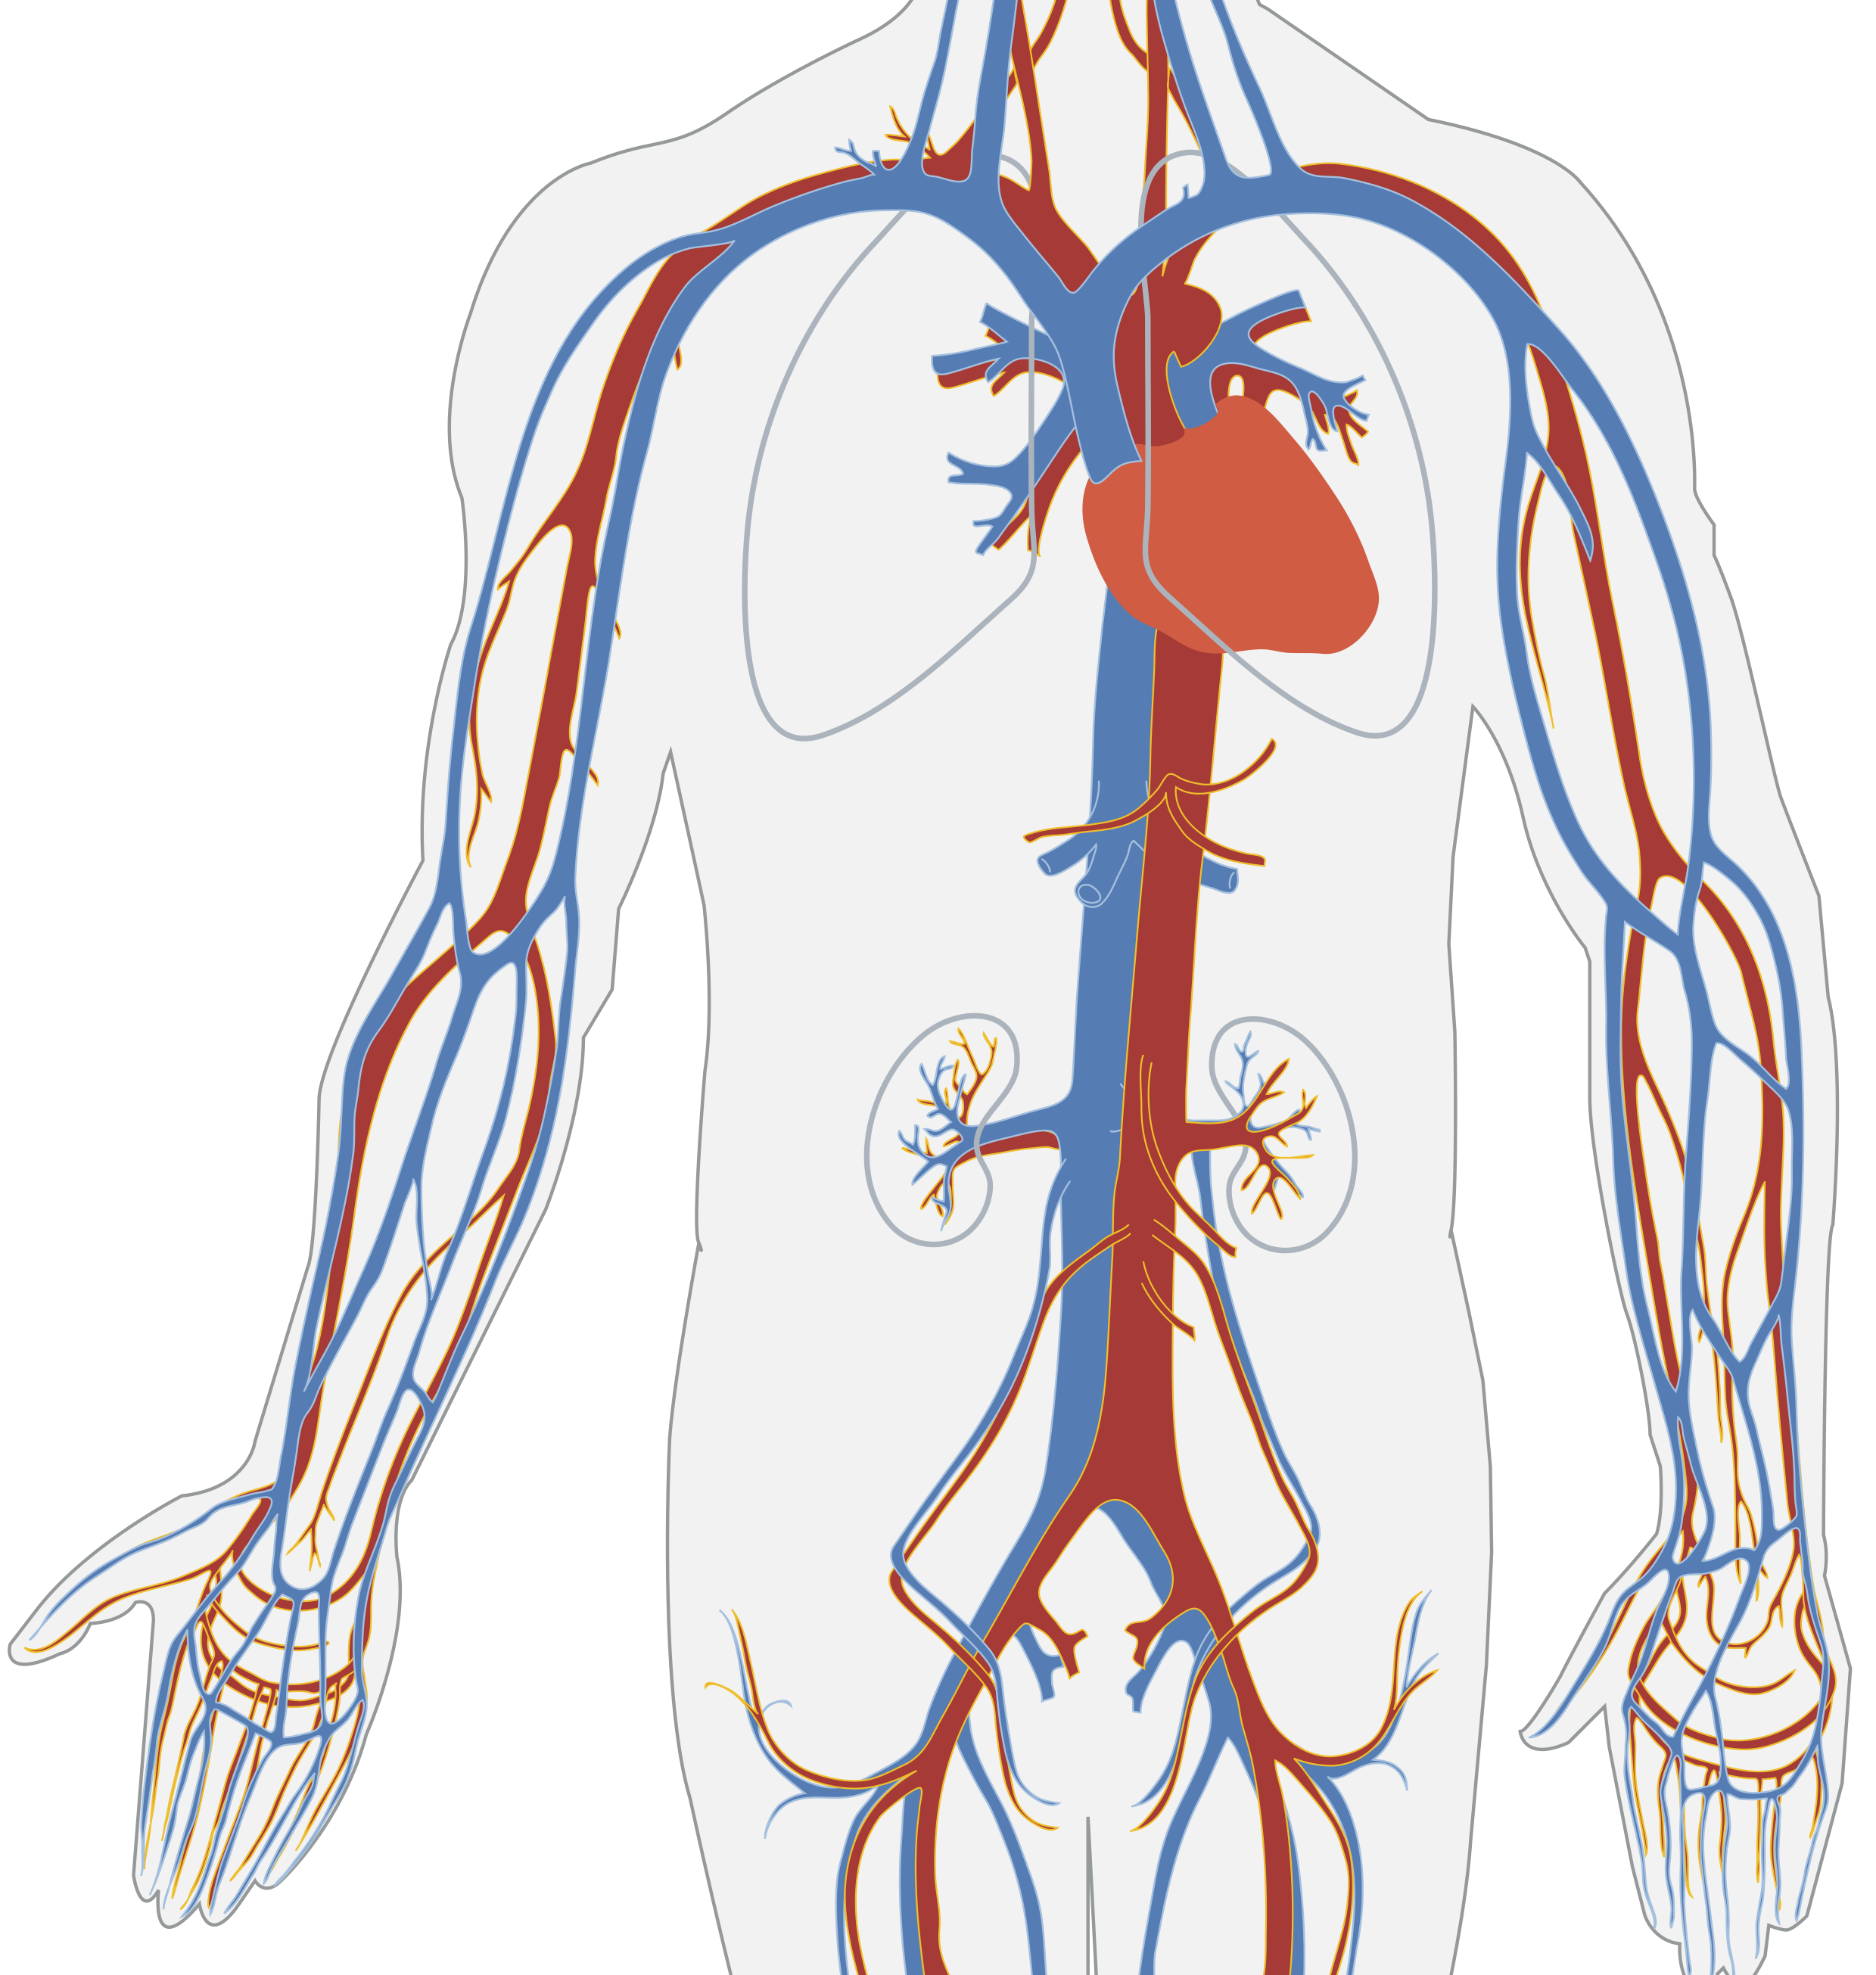
\includegraphics{ch1/Circulatory_System_no_tags_cropped.png}
\caption{Human blood circulates throughout the body and returns to the heart, veins shown in blue and arteries in red. \emph{Circulatory System en} by LadyofHats in public domain via Wikimedia Commons.}
\end{figure}

\hypertarget{galens-theory-of-blood}{%
\subsection{Galen's theory of blood}\label{galens-theory-of-blood}}

Galen came up with a different explanation based on the notion of \emph{humors}, or fluids, that was fundamental to the Greek conception of the body. He proposed that the venous and arterial blood were different humors: venous blood, or \emph{natural spirits}, was produced by the liver, while arterial blood, or \emph{vital spirits}, was produced by the heart and carried by the arteries, as shown in figure \ref{fig:galen_blood}. The heart consisted of two halves, and it warmed the blood and pushed both the natural and vital spirits out to the organs; the two spirits could mix through pores in the septum separating its right and left halves. The vital and natural spirits were both consumed by the organs, and regenerated by the liver and the heart. The purpose of the lungs was to serve as bellows, cooling the blood after it was heated by the heart.

\begin{figure}
\centering
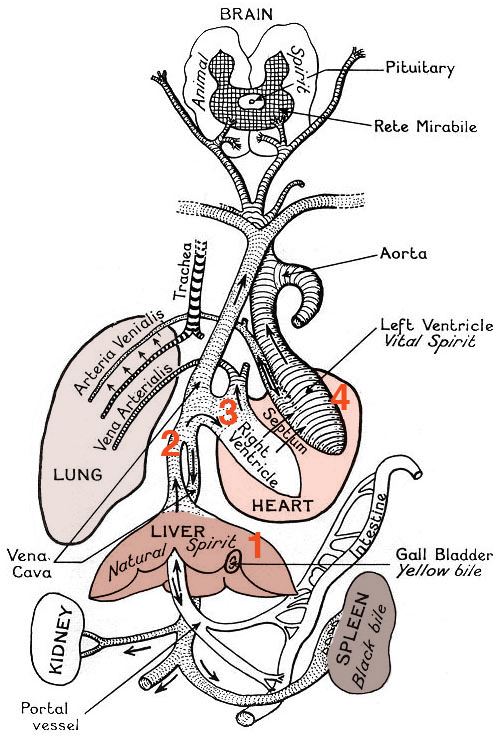
\includegraphics{ch1/galenheartc.png}
\caption{Illustration of Galen's conception of the blood system, showing different spirits traveling in one direction, but not circulating. Reproduced by permission of \href{https://faculty.humanities.uci.edu/bjbecker/}{Barbara Becker}.}
\end{figure}

Is this a good theory of how the heart, lungs, and blood work? Doctors in Europe thought so for over one thousand years! Galen's textbook on physiology was the standard for medical students through the 17th century. The theory seemed to make sense, and explain what was observable. Many great scientists and physicians, including Leonardo DaVinci and Avicenna, did not challenge the inaccuracies such as the porous septum in the heart, even though they could not see the pores themselves. It took both better observations and a quantitative testing of the hypothesis to challenge the orthodoxy.

\hypertarget{mathematical-testing-of-the-theory}{%
\subsection{Mathematical testing of the theory}\label{mathematical-testing-of-the-theory}}

William Harvey \index{Harvey, William} was born in England and studied medicine in Padua under the great physician Hieronymus Fabricius. He became famous, and would perform public demonstrations of physiology, using live animals for experiments that would not be approved today. He also studied the heart and the blood vessels, and measured the volume of the blood that can be contained in the human heart. He was quite accurate in estimating the correct volume, which we now know to be about 70 ml (1.5 oz). What is even more impressive is that he used this quantitative information to test Galen's theory.

Let us assume that all of the blood that is pumped out by the heart is consumed by the tissues, as Galen proposed; let us further assume that the heart beats at constant rate of 60 beats per minute, with a constant ejection volume of 70 ml. Then over the course of a day, the human body would consume about
\[\mathrm{Volume} = 70 \ \mathrm {mL} \times 60 \ \mathrm {(beats \ per \ minute)} \times 60 \ \mathrm {(minutes \ per \ hour)}  \times 24 \ \mathrm {(hours \ per \ day)}\]
or over 6,000 liters of blood! You may quibble over the exact numbers (some hearts beat faster or slower, some hearts may be larger or smaller) but the impact of the calculation remains the same: it is an absurd conclusion. Galen's theory would require the human being to consume and produce a quantity of fluid many times the volume of the human body (about 100 liters) in a day! This is a physical impossibility, so the only possible conclusion in that Galen's model is wrong.

This led Harvey to propose the \index{model!blood circulation}model that we know today: that blood is not consumed by the tissues, but instead returns to the heart and is re-used again \citep{schultz_william_2002}. This is why we call the heart and blood vessels part of the circulatory system of the body. This model was controversial at the time - some people proclaimed they would ``rather be wrong with Galen, than right with Harvey'\,' - but eventually became accepted as the standard model. What is remarkable is that Harvey's argument, despite being grounded in empirical data, was strictly mathematical. He adopted the assumptions of Galen, made the calculations, and got a result which was inconsistent with reality. This is an excellent example of how mathematical modeling can be useful, because it can provide clear evidence against a wrong hypothesis.

\hypertarget{sec:math1}{%
\section{Parameters and variables in models}\label{sec:math1}}

Many biologists remain skeptical of mathematical modeling. The criticism can be summarized like this: a theoretical model either agrees with experiment, or it does not. In the former case, it is useless, because the data are already known; in the latter case, it is wrong! As I indicated above, the goal of mathematical modeling is not to reproduce experimental data; otherwise, indeed, it would only be of interest to theoreticians. The correct question to ask is, does a theoretical model help us understand the real thing? There are at least three ways in which a model can be useful:

\begin{itemize}
\item
  A model can help a scientist make sense of complex data, by testing whether a particular mechanism explains the observations. Thus, a model can help clarify our understanding by throwing away the non-essential features and focusing on the most important ones.
\item
  A mathematical model makes predictions for situations that have not been observed. It is easy to change parameters in a mathematical model and calculate the effects. This can lead to new hypotheses that can be tested by experiments.
\item
  Model predictions can lead to better experimental design. Instead of trying a whole bunch of conditions, the theoretical model can suggest which ones will produce big effects, and thus can save a lot of work for the lab scientist.
\end{itemize}

In order to make a useful model of a complex living system, you have to simplify it. Even if you are only interested in a part of it, for instance a cell or a single molecule, you have to make simplifying choices. A small protein has thousands of atoms, a cell consists of millions of molecules, which all interact with each other; keeping track mathematically of every single component is daunting if not impossible. To build a useful mathematical model one must choose a few quantities which describe the system sufficiently to answer the questions of interest. For instance, if the positions of a couple of atoms in the protein you are studying determine its activity, those positions would make natural quantities to include in your model. You will find more specific examples of models later in this chapter.

Once you have decided on the essential quantities to be included in the model, these are divided into \index{variable!definition} \emph{variables} and \index{parameter} \emph{parameters}. As suggested by the name, a variable typically varies over time and the model tracks the changes in its value, while parameters usually stay constant, or change more slowly. However, that is not always the case. The most important difference is that variables describe quantities \textbf{within the system} being modeled, while parameters usually refer to quantities which are controlled by something \textbf{outside the system}.

As you can see from this definition, the same quantity can be a variable or a parameter depending on the scope of the model. Let's go back to our example of modeling a protein: usually the activity (and the structure) of a protein is influenced by external conditions such as pH and temperature; these would be natural parameters for a model of the molecule. However, if we model an entire organism, the pH (e.g.~of the blood plasma) and temperature are controlled by physiological processes within the organism, and thus these quantities will now be considered variables.

Perhaps the clearest way to differentiate between variables and parameters is to think about how you would present a data set visually. We will discuss plotting graphs of functions in chapter 2, and plotting data sets in chapter 3, but the reader has likely seen many such plots before. Consider which of the quantities you would to plot to describe the system you are modeling. If the quantity belongs on either axis, it is a variable, since it is important to describe how it changes. The rest of the quantities can be called parameters. Of course, depending on the question you ask, the same quantity may be plotted on an axis or not, which is why this classification is not absolute.

After we have specified the essential variables for your model, we can describe a complex and evolving biological system in terms of its \emph{state}. This is a very general term, but it usually means the values of all the variables that you have chosen for the model, which are often called \index{state!variable} \emph{state variables}. For instance, an ion channel can be described with the state variable of conformation, which may be in a open state or in a closed state. The range, or collection of all different states of the system is called the \index{state!space} \emph{state space} of the model. Below you will find examples of models of biological systems with diverse state spaces.

\hypertarget{discrete-state-variables-genetics}{%
\subsection{discrete state variables: genetics}\label{discrete-state-variables-genetics}}

There are genes which are present in a population as two different versions, called \index{allele}*alleles\} - let us use letters \(A\) and \(B\) to label them. One may describe the genetic state of an individual based on which allele it carries. If this individual is haploid, e.g.~a bacterium, then it only carries a single copy of the genome, and its state can be described by a single variable with the state space of \(A\) or \(B\).

A diploid organism, like a human, possesses two copies of each gene (unless it is on one of the sex chromosomes, X or Y); each copy may be in either state \(A\) or \(B\). This may seem to suggest that there are four different values in the genetic state space, but if the order of the copies does not matter (which is usually the case), then \(AB\) and \(BA\) are effectively the same, so the state space consists of three values: \(AA\), \(BB\), and \(AB\).

\hypertarget{discrete-state-variables-population}{%
\subsection{discrete state variables: population}\label{discrete-state-variables-population}}

Consider the model of a population of individuals, with the variable of number of individuals (populations size) and parameters being the birth and death rates. The state space of this model is \textbf{all integers between 0 and infinity.}

Consider the model of a population of individuals who may get infected. Assume that the total number of individuals does not change (that is, there are no births and deaths) and that these individuals can be in one of two states: healthy or sick (in epidemiology these are called \emph{susceptible} or \emph{infectious}). There are typically two parameters in such models: the probability of infection and the probability of recovery. Since the total population is fixed at some number \(N\), the space space of the model is all pairs of integers between 0 and \(N\) that add up to \(N\).

\hypertarget{continuous-state-variables-concentration}{%
\subsection{continuous state variables: concentration}\label{continuous-state-variables-concentration}}

Suppose that a biological molecule is produced with a certain rate and degraded with a different rate, and we would like to describe the quantity of the molecule, usually expressed as concentration. The relevant variables here are concentration and time, and you will see those variables on the axes of many plots in biochemistry. Concentration is a ratio of the number of molecules and the volume, so the state space can be any positive real number (although practically there is a limit as to how many molecules can fit inside a given volume, but for simplicity we can ignore this).

Going even further, let us consider an entire cell, which contains a large number of different molecules. We can describe the state of a cell as the collection of all the molecular concentrations, with the parameters being the rates of all the reactions going on between those molecules. The state space for this model with \(N\) different molecules is \(N\) positive real numbers.

\hypertarget{multiple-variables-in-medicine}{%
\subsection{multiple variables in medicine}\label{multiple-variables-in-medicine}}

Doctors take medical history from patients and measure vital signs to get a picture of a patient's health. These can be all be thought of as variables in a model of a person that physicians construct. Some of these variables are discrete, for instance whether there is family history of hypertension, which has only two values: yes or no. Other variables are numbers with a range, such as weight and blood pressure. The state space of this model is a combination of \emph{categorical} values (such as yes/no) and \emph{numerical} values (within a reasonable range).

\hypertarget{discussion-questions}{%
\subsection{Discussion questions}\label{discussion-questions}}

Several biological models are indicated below. Based on what you know, divide the quantities into variables and parameters and describe the state space of the model. Note that there may be more than one correct interpretation

\begin{enumerate}
\def\labelenumi{\arabic{enumi}.}
\item
  The volume of blood pumped by the heart over a certain amount of time, depending on the heart rate and the ejection volume.
\item
  The number of wolves in a national forest depending on the number of wolves in the previous year, the birth rate, the death rate, and the migration rate.
\item
  The fraction of hemes in hemoglobin (a transport protein in red blood cells) which are bound to oxygen depending on the partial pressure of oxygen and the binding cooperativity of hemoglobin.
\item
  The number of mutations that occur in a genome, depending on the mutation rate, the amount of time, and the length of the genome.
\item
  The concentration of a drug in the blood stream depending on the dose, time after administration, and the rate of metabolism (processing) of the drug.
\item
  Describing an outbreak of an infectious disease in a city in terms of the fractions of infected, healthy, and recovered people, depending on the rate of infection, rate of recovery, and the mortality rate of the disease.
\end{enumerate}

\hypertarget{first-steps-in-r}{%
\section{First steps in R}\label{first-steps-in-r}}

\label{sec:comp1}
A central goal of this book is to help you, the reader, gain experience with computation, which requires learning some programming (cool kids call it ``coding''). Programming is a way of interacting with computers through a symbolic language, unlike the graphic user interfaces that we're all familiar with. Basically, programming allows you to make a computer do exactly what you want it to do.

There is a vast number of computer languages with distinct functionalities and personalities. Some are made to talk directly to the computer's ``brain'' (CPU and memory), e.g.~Assembly, while others are better suited for human comprehension, e.g.~python or Java. Programming in any language involves two parts: 1) writing a program (code) using the commands and the syntax for the language; 2) running the code by using a compiler or interpreter to translate the commands into machine language and then making the computer execute the actions. If your code has a mistake in it, the compiler or interpreter should catch it, and return an \emph{error message} to you instead of executing the code. Sometimes, though, the code may pass muster with the interpreter/compiler, but it may still have a mistake (bug). This can be manifested in two different ways: either the code execution does not produce the result that you intended, or it hangs up or crashes the computer (the latter is hard to do with the kind of programming we will be doing). We will discuss errors and how to prevent and catch these bugs as you develop your programming skills.

In this course, our goal is to compute mathematical models and to analyze data, so we choose a language that is designed specially for these tasks, which is called R. To proceed, you'll need to download and install R, which is freely available \href{cran.r-project.org/}{here}. In addition to downloading the language (which includes the interpreter that allows you to run R code on your computer) you will need to download a graphic interface for writing, editing, and running R code, called R Studio (coders call this an IDE, or an Integrated Developer Environment), which is also free and available \href{www.rstudio.com/products/rstudio/download/}{here}.

\hypertarget{r-markdown-and-r-studio}{%
\subsection{R Markdown and R Studio}\label{r-markdown-and-r-studio}}

In this course you will use R using R Studio and R Markdown documents, which are text files with the extension \texttt{.Rmd}. Markdown is a simple formatting syntax for creating reports in HTML, PDF, or Word format by incorporating text with code and its output. More details on using R Markdown are \href{rmarkdown.rstudio.com}{here}. In fact, this whole book is written in R Markdown files and then compiled to produce the beautiful (I hope you agree) web book that you are reading.

If you open an Rmd file in R Studio, you will see a \textbf{Knit} button on top of the Editor window. Clicking it initiates the processing of the file into an output document (in HTML, PDF, or Word format) that includes the text as well as the output of any embedded R code chunks within the document. You can embed an R \emph{code chunk} like this:

\begin{Shaded}
\begin{Highlighting}[]
\KeywordTok{print}\NormalTok{(}\StringTok{"Hello there!"}\NormalTok{) }
\end{Highlighting}
\end{Shaded}

\begin{verbatim}
## [1] "Hello there!"
\end{verbatim}

To run the code inside a single R code chunk, click the green arrow in the top right of the chunk. This will produce an output, in this case the text ``Hello there!''. Inside the generated output file, for example the web book you may be reading, the output of code chunks is shown below the box with the R code and indicated by two hashtags.

You can make text \textbf{bold} or \emph{italic} like so. You can also use mathematical notation called LaTeX, which you'll see used below to generate nice-looking equations. LaTeX commands are surrounded by dollar signs, for example \$e\^{}x\$ generates \(e^x\). Mathematical types love LaTeX, but you can use R Markdown without it.

\hypertarget{numbers-and-arithmetic-operations}{%
\subsection{numbers and arithmetic operations}\label{numbers-and-arithmetic-operations}}

When you get down to the brass tacks, all computation rests on performing \index{R programming!arithmetic} \emph{arithmetic operations}: addition, subtraction, multiplication, division, exponentiation, etc. The symbols used for arithmetic operations are what you'd expect: \texttt{+}, \texttt{-}, \texttt{*}, \texttt{/} are the four standard operations, and \texttt{\^{}} is the symbol for exponentiation. For example, type \texttt{2\^{}3} in any R code chunk and execute it:

\begin{Shaded}
\begin{Highlighting}[]
\DecValTok{2}\OperatorTok{\^{}}\DecValTok{3}
\end{Highlighting}
\end{Shaded}

\begin{verbatim}
## [1] 8
\end{verbatim}

You see that R returns the result by printing it out on the screen. The number in square brackets {[}1{]} is not important for now; it is useful when the answer contains many numbers and has to be printed out on many rows. The second number is the result of the calculation.

For numbers that are either very large or very small, it's too cumbersome to write out all the digits, so R, like most computational platforms, uses the \index{R programming!scientific notation}\emph{scientific notation}. For instance, if you want to represent 1.4 billion, you type in the following command; note that 10 to the ninth power is represented as \texttt{e+09} and the prefix 1.4 is written without any multiplication sign:

\begin{Shaded}
\begin{Highlighting}[]
\FloatTok{1.4}\OperatorTok{*}\DecValTok{10}\OperatorTok{\^{}}\DecValTok{9}
\end{Highlighting}
\end{Shaded}

\begin{verbatim}
## [1] 1.4e+09
\end{verbatim}

There are also certain numbers built into the R language, most notably \(\pi\) and \(e\), which can be accessed as follows:

\begin{Shaded}
\begin{Highlighting}[]
\NormalTok{pi}
\end{Highlighting}
\end{Shaded}

\begin{verbatim}
## [1] 3.141593
\end{verbatim}

\begin{Shaded}
\begin{Highlighting}[]
\KeywordTok{exp}\NormalTok{(}\DecValTok{1}\NormalTok{)}
\end{Highlighting}
\end{Shaded}

\begin{verbatim}
## [1] 2.718282
\end{verbatim}

The expression \texttt{exp()} is an example of a function, which we will discuss in section \ref{sec:comp2}; it returns the value of \(e\) raised to the power of the number in parenthesis, hence \texttt{exp(1)} returns \(e\). Notice that although both numbers are irrational, and thus have infinitely many decimal digits, R only prints out a few of them. This doesn't mean that it doesn't have more digits in memory, but it only displays a limited number to avoid clutter. The number of digits to be displayed can be changed, for example to display 10 digits, type in \texttt{options(digits=10)}.

Computers are very good at computation, as their name suggests, but they have limitations. In order to manipulate numbers, they must be stored in computer memory, but computer memory is finite. There is a limit to the length of the number that is feasible to store on a computer. This has implications for both very large numbers and to very small numbers, which are close to zero, because both require many digits for storage.

All programming languages have an upper limit on the biggest number it will store and work with. If an arithmetic operation results in a number larger than that limit, the computer will call it an \emph{overflow} error. Depending on the language, this may stop the execution of the program, or else produce a non-numerical value, such as \texttt{NaN} (not a number) or \texttt{Inf} (infinite). Do exercise \ref{ex:overflow} to investigate the limitations of R for large numbers.

On the other hand, very small numbers present their own challenges. As with very large numbers, a computer cannot store an arbitrary number of digits after the decimal (or binary) point. Therefore, there is also the smallest number that a programming language will accept and use, and storing a smaller number produces an \emph{underflow} error. This will either cause the program execution to stop, or to return the value 0 instead of the correct answer. Do exercise \ref{ex:underflow} to investigate the limitations of R for small numbers.

This last fact demonstrates that all computer operations are imprecise, as they are limited by what's called the \index{R programming!machine precision} \emph{machine precision}, which is illustrated in exercise \ref{ex:mach_prec}. For instance, two similar numbers, if they are within the machine precision of one another, will be considered the same by the computer. Modern computers have large memories, and their machine precision is very good, but sometimes this error presents a problem, e.g.~when subtracting two numbers. A detailed discussion of machine error is beyond the scope of this text, but anyone performing computations must be aware of its inherent limitations.

\hypertarget{r-coding-exercises}{%
\subsection{R Coding Exercises}\label{r-coding-exercises}}

\begin{enumerate}
\def\labelenumi{\arabic{enumi}.}
\item
  Calculate the value of \(\pi\) raised to the 10th power.
\item
  Use the scientific notation to multiply four billion by \(\pi\).
\item
  Use the scientific notation with large exponents (e.g.~1e+100, 1e+500, etc.) to find out what happens when you give R a number that is too large for it to handle. Approximately at what order of magnitude does R produce an overflow error?
\item
  In the same fashion, find out what happens when you give R a number that is too small for it to handle. Approximately at what order of magnitude does R produce an underflow error?
\item
  How close can two numbers be before R thinks they are the same? Subtract two numbers which are close to each other, like 24 and 24.001, and keep making them closer to each other, until R returns a difference of zero. Report at what value of the actual difference this happens.
\end{enumerate}

\hypertarget{variable-assignment}{%
\subsection{variable assignment}\label{variable-assignment}}

Variables in programming languages are used to store and access numerical or other information. After \index{variable!assignment}\emph{assigning}\} it a value for the first time (\emph{initializing}), a variable name can be used to represent the value we assigned to it. Invoking the name of variable recalls the stored value from computer's memory. There are a few rules about naming variables: a name cannot be a number or an arithmetic operator like \texttt{+}, in fact it cannot contain symbols for operators or spaces inside the name, or else confusion would reign. Variable names may contain numbers, but not as the first character. When writing code it is good practice to give variables informative names, like \emph{height} or \emph{city\_pop}. \index{R programming!variable assignment}

The symbol `=' is used to assign a value to a variable in most programming languages, and can be used in R too. However, it is customary for R to use the symbols \texttt{\textless{}-} together to indicate assignment, like this:

\begin{Shaded}
\begin{Highlighting}[]
\NormalTok{var1 \textless{}{-}}\StringTok{ }\DecValTok{5}
\end{Highlighting}
\end{Shaded}

After this command the variable \texttt{var1} has the value 5, which you can see in the upper right frame in R Studio called \emph{Environment}. In order to display the value of the variable as an output on the screen, use the special command \texttt{print()} (it's actually a function, which we will discuss in the next chapter). The following two commands show that the value of a variable can be changed after it has been initialized:

\begin{Shaded}
\begin{Highlighting}[]
\NormalTok{var1 \textless{}{-}}\StringTok{ }\DecValTok{5}
\NormalTok{var1 \textless{}{-}}\StringTok{ }\DecValTok{6}
\KeywordTok{print}\NormalTok{(var1)}
\end{Highlighting}
\end{Shaded}

\begin{verbatim}
## [1] 6
\end{verbatim}

While seemingly contradictory, the commands are perfectly clear to the computer: first \texttt{var1} is assigned the value 5 and then it is assigned 6. After the second command, the first value is forgotten, so any operations that use the variable \texttt{var1} will be using the value of 6.

Entire expressions can be placed on the right hand side of an assignment command: they could be arithmetic or logical operations as well as functions, which we will discuss later on. For example, the following commands result in the value 6 being assigned to the variable \texttt{var2}:

\begin{Shaded}
\begin{Highlighting}[]
\NormalTok{var1 \textless{}{-}}\StringTok{ }\DecValTok{5}
\NormalTok{var2 \textless{}{-}}\StringTok{ }\NormalTok{var1}\OperatorTok{+}\DecValTok{1}
\KeywordTok{print}\NormalTok{(var2)}
\end{Highlighting}
\end{Shaded}

\begin{verbatim}
## [1] 6
\end{verbatim}

Even more mind-blowing is that the same variable can be used on both sides of an assignment operator! The R interpreter first looks on the right hand side to evaluate the expression and then assigns the result to the variable name on the left hand side. So for instance, the following commands increase the value of \texttt{var1} by 1, and then assign the product of \texttt{var1} and \texttt{var2} to the variable \texttt{var2}:

\begin{Shaded}
\begin{Highlighting}[]
\NormalTok{var1 \textless{}{-}}\StringTok{ }\NormalTok{var1 }\OperatorTok{+}\StringTok{ }\DecValTok{1}
\KeywordTok{print}\NormalTok{(var1)}
\end{Highlighting}
\end{Shaded}

\begin{verbatim}
## [1] 6
\end{verbatim}

\begin{Shaded}
\begin{Highlighting}[]
\NormalTok{var2 \textless{}{-}}\StringTok{ }\NormalTok{var1}\DecValTok{{-}1}
\KeywordTok{print}\NormalTok{(var2)}
\end{Highlighting}
\end{Shaded}

\begin{verbatim}
## [1] 5
\end{verbatim}

\begin{Shaded}
\begin{Highlighting}[]
\NormalTok{var2 \textless{}{-}}\StringTok{ }\NormalTok{var1}\OperatorTok{*}\NormalTok{var2}
\KeywordTok{print}\NormalTok{(var2)}
\end{Highlighting}
\end{Shaded}

\begin{verbatim}
## [1] 30
\end{verbatim}

We have seen example of how to assign values to variables, so here is an example of how NOT to assign values, with the resulting error message:

\begin{Shaded}
\begin{Highlighting}[]
\NormalTok{var1 }\OperatorTok{+}\StringTok{ }\DecValTok{1}\NormalTok{ \textless{}{-}}\StringTok{ }\NormalTok{var1}
\end{Highlighting}
\end{Shaded}

The left-hand side of an assignment command should contain only the variable to which you are assigning a value, not an arithmetic expression to be performed.

\hypertarget{r-coding-exercises-1}{%
\subsection{R Coding Exercises}\label{r-coding-exercises-1}}

The following commands or scripts do not work as intended. Find the errors and correct them, then run them to make sure they do what they are intended to do:

\hypertarget{exercises}{%
\subsection{Exercises:}\label{exercises}}

The following R commands or short scripts contain errors; your job is to fix them so they runs as described. (Remove the \# at the start of each line to ``uncomment'' the code first.)

\begin{enumerate}
\def\labelenumi{\arabic{enumi}.}
\tightlist
\item
  Assign the value -10 to a variable
\end{enumerate}

\begin{Shaded}
\begin{Highlighting}[]
\NormalTok{neg {-}\textgreater{}}\StringTok{ }\DecValTok{{-}10}
\end{Highlighting}
\end{Shaded}

\begin{enumerate}
\def\labelenumi{\arabic{enumi}.}
\setcounter{enumi}{1}
\tightlist
\item
  Assign a variable the value 5 and then increase its value by 3:
\end{enumerate}

\begin{Shaded}
\begin{Highlighting}[]
\NormalTok{2pac \textless{}{-}}\StringTok{ }\DecValTok{5}
\NormalTok{2pac \textless{}{-}}\StringTok{ }\NormalTok{2pac }\OperatorTok{+}\StringTok{ }\DecValTok{3}
\end{Highlighting}
\end{Shaded}

\begin{enumerate}
\def\labelenumi{\arabic{enumi}.}
\setcounter{enumi}{2}
\tightlist
\item
  Assign the values 4 and 7 to two variables, then add them together and assign the sum to a new variable:
\end{enumerate}

\begin{Shaded}
\begin{Highlighting}[]
\NormalTok{total \textless{}{-}}\StringTok{ }\NormalTok{part1 }\OperatorTok{+}\StringTok{ }\NormalTok{part2}
\NormalTok{part1 \textless{}{-}}\StringTok{ }\DecValTok{4}
\NormalTok{part2 \textless{}{-}}\StringTok{ }\DecValTok{7}
\end{Highlighting}
\end{Shaded}

\begin{enumerate}
\def\labelenumi{\arabic{enumi}.}
\setcounter{enumi}{3}
\tightlist
\item
  Add 5 and 3 and save it into variable my.number
\end{enumerate}

\begin{Shaded}
\begin{Highlighting}[]
\DecValTok{5} \OperatorTok{+}\StringTok{ }\DecValTok{3}\NormalTok{ \textless{}{-}}\StringTok{ }\NormalTok{my.number}
\end{Highlighting}
\end{Shaded}

\begin{enumerate}
\def\labelenumi{\arabic{enumi}.}
\setcounter{enumi}{4}
\tightlist
\item
  Print the value of my.number on the screen:
\end{enumerate}

\begin{Shaded}
\begin{Highlighting}[]
\NormalTok{print[my.number]}
\end{Highlighting}
\end{Shaded}

\begin{enumerate}
\def\labelenumi{\arabic{enumi}.}
\setcounter{enumi}{5}
\tightlist
\item
  Replace the value of my.number with 5 times its current value
\end{enumerate}

\begin{Shaded}
\begin{Highlighting}[]
\NormalTok{my.number \textless{}{-}}\StringTok{ }\NormalTok{5my.number }
\end{Highlighting}
\end{Shaded}

\begin{enumerate}
\def\labelenumi{\arabic{enumi}.}
\setcounter{enumi}{6}
\tightlist
\item
  Assign the values of 7 and 8 to variables a and b, respectively, multiply them and save the results in variable x
\end{enumerate}

\begin{Shaded}
\begin{Highlighting}[]
\NormalTok{a\textless{}{-}}\DecValTok{7}
\NormalTok{b\textless{}{-}}\DecValTok{8}
\NormalTok{x\textless{}{-}ab}
\KeywordTok{print}\NormalTok{(x)}
\end{Highlighting}
\end{Shaded}

\begin{enumerate}
\def\labelenumi{\arabic{enumi}.}
\setcounter{enumi}{8}
\tightlist
\item
  Assign the value 42 to a variable, then increase it by 1
\end{enumerate}

\begin{Shaded}
\begin{Highlighting}[]
\NormalTok{age \textless{}{-}}\StringTok{ }\DecValTok{42}
\NormalTok{age }\OperatorTok{+}\StringTok{ }\DecValTok{1}\NormalTok{ \textless{}{-}}\StringTok{ }\NormalTok{age}
\end{Highlighting}
\end{Shaded}

\begin{enumerate}
\def\labelenumi{\arabic{enumi}.}
\setcounter{enumi}{8}
\tightlist
\item
  Assign the value 10 to variable radius, then calculate the area of the circle with that radius using the formula \(A = \pi r^2\):
\end{enumerate}

\begin{Shaded}
\begin{Highlighting}[]
\NormalTok{r \textless{}{-}}\StringTok{ }\DecValTok{10}
\NormalTok{area \textless{}{-}}\StringTok{ }\NormalTok{pir}\OperatorTok{\^{}}\DecValTok{2} 
\end{Highlighting}
\end{Shaded}

\hypertarget{functions-and-their-graphs}{%
\chapter{Functions and their graphs}\label{functions-and-their-graphs}}

\begin{quote}
Some fathers, if you ask them for the time of day, spit silver dollars.\\
Donald Barthelme, \emph{The Dead Father}
\end{quote}

Mathematical models describe how various quantities affect each other. In the last chapter we learned that these descriptions can be written down, often in the form of an equation. For instance, we can describe the total volume of blood pumped over a period of time as the product of stroke volume, the heart rate and the number of minutes, which can be written as an equation. The different quantities have their own meaning and roles, depending on what they stand for. To better describe how these quantities are related we use the deep idea of mathematical functions. In this chapter you will learn to do the following:

\begin{itemize}
\tightlist
\item
  use dimensional analysis to deduce the meaning of quantities in a model
\item
  understand the concept of function, dependent and independent variables
\item
  recognize basic functional forms and the shape of their graphs
\item
  use R to plot functions
\item
  understand basic models of reaction rates
\end{itemize}

\hypertarget{sec:model2}{%
\section{Dimensions of quantities}\label{sec:model2}}

What distinguishes a mathematical model from a mathematical equation is that the quantities involved have a real-world meaning. Each quantity represents a measurement, and associated with each one are the \index{units} \emph{units} of measurement. The number 173 is not enough to describe the height of a person - you are left to wonder 173 what? meters, centimeters, nanometers, light-years? Obviously, only centimeters make sense as a unit of measurement for human height; but if we were measuring the distance between two animals in a habitat, meters would be a reasonable unit, and it were the distance between molecules in a cell, we would use nanometers. Thus, any quantity in a mathematical model must have associated units, and any graphs of these quantities must be labeled accordingly.

In addition to units, each variable and parameter has a meaning, which is called the \index{dimension} \emph{dimension} of the quantity. For example, any measurement of length or distance has the same dimension, although the units may vary. The value of a quantity depends on the units of measurement, but its essential dimensionality does not. One can convert a measurement in meters to that in light-years or cubits, but one cannot convert a measurement in number of sheep to seconds - that conversion has no meaning.

Thus leads us to the fundamental rule of mathematical modeling: \textbf{terms that are added or subtracted must have the same dimension}. This gives mathematical modelers a useful tool called \index{dimensional analysis} \emph{dimensional analysis}, which involves replacing the quantities in an equation with their dimensions. This serves as a check that all dimensions match, as well as allowing to deduce the dimensions of any parameters for which the dimension was not specified. \citep{smith_mathematical_1968}

\textbf{Example.} As we saw in chapter 1, the relationship between the amount blood pumped by a heart in a certain amount of time is expressed in the following equation, where \(V_{tot}\) and \(V_s\) are the total volume and stroke volume, respectively, \(R\) is the heart rate, and \(t\) is the time:
\[
V_{tot} = V_sRt
\]
The dimension of a quantity \(X\) is denoted by \([X]\); for example, if \(t\) has the dimension of time, we write \([t] = time\). The dimension of volume is \([V_{tot}] = length^3\), the dimension of stroke volume is \([V_s] = volume/beat\) and the dimension of time \(t\) is time, so we can re-write the equation above in dimensional form:

\[length^3 = length^3/ beat \times R \times time\]

Solving this equation for R, we find that it must have the dimensions of \([R] = beats/time\). It can be measured in beats per minute (typical for heart rate), or beats per second, beats per hour, etc. but the
\emph{dimensionality} of the quantity cannot be changed without making the model meaningless.

There are also \index{dimensionless quantity} \emph{dimensionless} quantities, or pure numbers, which are not tied to a physical meaning at all. Fundamental mathematical constants, like \(\pi\) or \(e\), are classic examples, as are some important quantities in physics, like the Reynolds number in fluid mechanics. \citep{strogatz_nonlinear_2001} Quantities with a dimension can be made dimensionless by dividing them by another quantity with the same dimension and ``canceling'' the dimensions. For instance, we can express the height of a person as a fraction of the mean height of the population; then the height of a tall person will become a number greater than 1, and the height of a short one will become less than 1. This new dimensionless height does not have units of length - they have been divided out by the mean height. This is known as \index{rescaling} \emph{rescaling} the quantity, by dividing it by a preferred scale. There is a fundamental difference between rescaling and changing the units of a quantity: when changing the units, e.g.~from inches to centimeters, the dimension remains the same, but if one divides the quantity by a scale, it loses its dimension.

\textbf{Example.} The model for a population of bacteria that doubles every hour is described by the equation, where \(P_0\) is initial number of bacteria and \(P\) is the population after \(t\) hours:
\[ P = P_0 2^t \]
Let us define the quantity \(R=P/P_0\), so we can say that population increased by a factor of \(R\) after \(t\) hours. This ratio is a dimensionless quantity because \(P\) and \(P_0\) have the same dimension of bacterial population, which cancel out. The equation for \(R\) can be written as follows:
\[ R= 2^t \]
According to dimensional analysis, both sides of the equation have to be dimensionless, so \(t\) must also be a dimensionless variable. This is surprising, because \(t\) indicates the number of hours the bacterial colony has been growing. This reveals the subtle fact that \(t\) is a rescaled variable obtained by dividing the elapsed time by the length of the reproductive cycle. Because of the assumption that the bacteria divide exactly once an hour, \(t\) counts the number of hours, but if they divided once a day, \(t\) would denote the number of days. So \(t\) doesn't have units or dimensions, but instead denotes the dimensionless number of cell divisions.

\hypertarget{exercises}{%
\subsection{Exercises}\label{exercises}}

For each biological model below determine the dimensions of the parameters, based on the given dimensions of the variables.

\begin{enumerate}
\def\labelenumi{\arabic{enumi}.}
\item
  Model of number of mutations \(M\) as a function of time \(t\):
  \[ M(t) = M_0 + \mu t\]
\item
  Model of molecular concentration \(C\) as a function of time \(t\):
  \[ C(t) = C_0 e^{-kt} \]
\item
  Model of tree height \(H\) (length) as a function of age \(a\) (time):
  \[ H(a) = \frac{b a}{c + a}\]
\item
  Model of cooperative binding of ligands, with fraction of bound receptors \(\theta\) as a function of ligand concentration \(L\):
  \[ \theta (L) = \frac{L^n}{L^n + K_d}\]
\item
  Model of concentration of a gene product \(G\) (concentration) as a function of time \(t\):
  \[ G(t) = G_m (1 - e^{-\alpha t})\]
\item
  Michaelis-Menten model of enzyme kinetics, \(v\) is reaction rate (1/time) and \(S\) is substrate concentration:
  \[ v(S) = \frac{v_{max} S}{K_m + S}\]
\item
  Logistic model of population growth, \(P\) is population size and time \(t\):
  \[ P(t) = \frac{A e^{kt}}{1 + B(e^{kt} -1)} \]
\end{enumerate}

\hypertarget{sec:math2}{%
\section{Functions and their graphs}\label{sec:math2}}

A relationship between two variables addresses the basic question: when one variable changes, how does this affect the other? An equation, like the examples in the last section, allows one to calculate the value of one variable based on the other variable and parameter values. In this section we seek to describe more broadly how two variables are related by using the mathematical concept of functions.

\textbf{Definition:} A \index{function!mathematical} function is a mathematical rule which has an input and an output. A function returns a well-defined output for every input, that is, for a given input value the function returns a unique output value.

In this abstract definition of a function it doesn't have to be written as an algebraic equation, it only has to return a unique output for any given input value. In mathematics we usually write them down in terms of algebraic expressions. As in mathematical models, you will see two different kinds of quantities in equations that define functions: variables and parameters. The input and the output of a function are usually variables, with the input called the \index{variable!independent} \emph{independent variable} and the output called the \index{variable!dependent} \emph{dependent variable}.

The relationship between the input and the output can be graphically illustrated in a \index{function!graph} graph, which is a collection of paired values of the independent and dependent variable drawn as a curve in the plane. Although it shows how the two variables change relative to each other, parameters may change too, which results in a different graph of the function. While graphing calculators and computers can draw graphs for you, it is very helpful to have an intuitive understanding about how a function behaves, and how the behavior depends on the parameters. Here are the three questions to help picture the relationship (assume \(x\) is the independent variable and it is a nonnegative real number):

\begin{enumerate}
\def\labelenumi{\arabic{enumi}.}
\tightlist
\item
  what is the value of the function at \(x=0\)?
\item
  what does the function do when \(x\) becomes large (\(x \to \infty\))?
\item
  what does the function do between the two extremes?
\end{enumerate}

Below you will find examples of fundamental functions used in biological models with descriptions of how their parameters influence their graphs.

\hypertarget{linear-and-exponential-functions}{%
\subsection{linear and exponential functions}\label{linear-and-exponential-functions}}

The reader is probably familiar with linear and exponential functions from algebra courses. However, they are so commonly used that it is worth going over them to refresh your memory and perhaps to see them from another perspective.

\label{def:ch2_linfunk}
\textbf{Definition} A \index{function!linear}\index{linear!function} linear function \(f(x)\) is one for which the difference in two function values is the same for a specific difference in the independent variable.

In mathematical terms, this can be written an equation for any two values of the independent variable \(x_1\) and \(x_2\) and a difference \(\Delta x\):

\[ f(x_1 + \Delta x) - f(x_1) = f(x_2 + \Delta x) - f(x_2) \]
The general form of the linear function is written as follows:
\begin{equation}
f(x) = ax + b
\label{eq:linear_funk}
\end{equation}

The function contains two parameters: the \index{slope!linear function}\index{linear!slope} slope \(a\) and the \index{y-intercept!linear function} y-intercept \(b\). The graph of the linear function is a line (hence the name) and the slope \(a\) determines its steepness. A positive slope corresponds to the graph that increases as \(x\) increases, and a negative slope corresponds to a declining function. At \(x=0\), the function equals \(b\), and as \(x \to \infty\), the function approaches positive infinity if \(a>0\), and approaches negative infinity if \(a<0\).

\label{def:ch2_expfunk}
\textbf{Definition} An \index{exponential!function}\index{function!exponential}exponential function \(f(x)\) is one for which the ratio of two function values is the same for a specific difference in the independent variable.

Mathematically speaking, this can be written as follows for any two values of the independent variable \(x_1\) and \(x_2\) and a difference \(\Delta x\):
\[ \frac{f(x_1 + \Delta x)}{f(x_1)} = \frac{f(x_2 + \Delta x)}{f(x_2)}\]

Exponential functions can be written using different symbolic forms, but they all have a constant base with the variable \(x\) in the exponent. I prefer to use the constant \(e\) (base of the natural logarithm) as the base of all the exponential functions, for reasons that will become apparent in chapter 15. This does not restrict the range of possible functions, because any exponential function can be expressed using base \(e\), using a transformation: \(a^x = e^{x \ln(a)}\). So let us agree to write exponential functions in the following form:
\begin{equation}
 f(x) = a e^{rx}
\label{eq:exp_funk}
\end{equation}

The function contains two parameters: the \index{exponential!rate constant}\emph{rate constant} \(r\) and the multiplicative constant \(a\). The graph of the exponential function is a curve which crosses the y-axis at \(y=a\) (plug in \(x=0\) to see that this is the case). As \(x\) increases, the behavior of the graph depends on the sign of the rate constant \(r\). If \(r>0\), the function approaches infinity (positive if \(a>0\), negative if \(a<0\)) as \(x \to \infty\). If \(r<0\), the function decays at an ever-decreasing pace and asymptotically approaches zero as \(x \to \infty\). Thus the graph of \(f(x)\) is a curve either going to infinity or a curve asymptotically approaching 0, and the steepness of the growth or decay is determined by \(r\).

\begin{figure}

{\centering 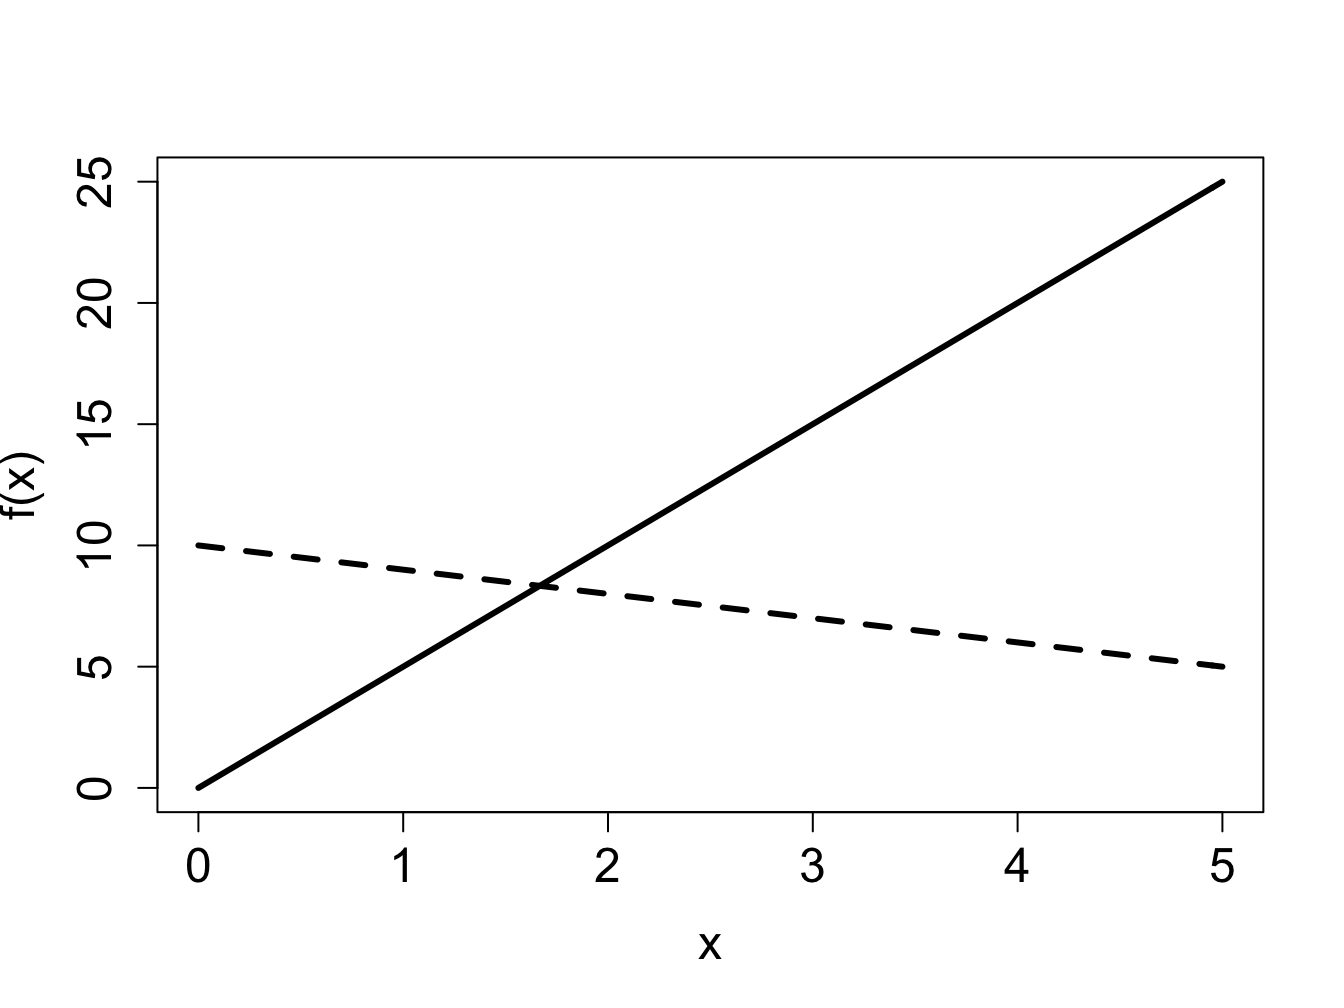
\includegraphics[width=0.5\linewidth]{QuantLife_files/figure-latex/ch2-funk1-1} 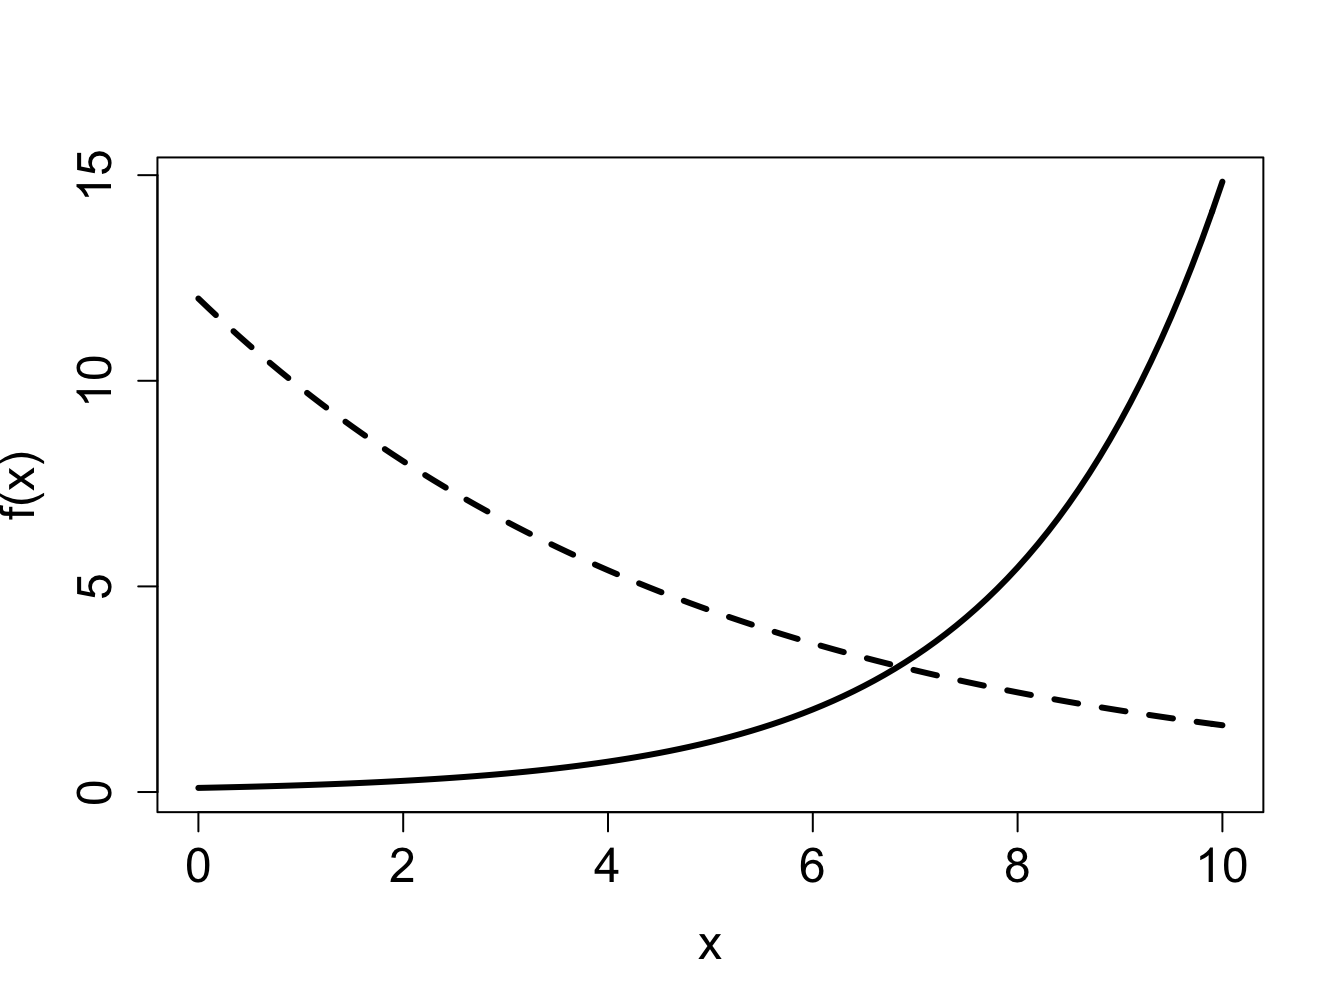
\includegraphics[width=0.5\linewidth]{QuantLife_files/figure-latex/ch2-funk1-2} 

}

\caption{Plots of two linear functions (left) and two exponential functions (right). Can you identify which linear function has the positive slope and which one negative? Which exponential function has a positive rate constant and which one negative?}\label{fig:ch2-funk1}
\end{figure}

\hypertarget{exercises-1}{%
\subsection{Exercises}\label{exercises-1}}

Answer the questions below, some of which refer to the function graphs in figure \ref{ch2-funk1}.

\begin{enumerate}
\def\labelenumi{\arabic{enumi}.}
\item
  Which of the linear graphs in the first figure corresponds to \(f(x) = 5x\) and which corresponds to \(f(x) = 10-x\)? State which parameter allows you to connect the function with its graph and explain why.
\item
  Which of the exponential graphs in the second figure corresponds to \(f(x) = 0.1e^{0.5x}\) and which corresponds to \(f(x) = 12e^{-0.2x}\)? State which parameter allows you to connect the function with its graph and explain why.
\item
  Demonstrate algebraically that a linear function of the form given in equation \ref{eq:linear_funk} satisfies the property of linear functions from definition \ref {def:ch2_linfunk}.
\item
  Demonstrate algebraically that an exponential function of the form given in equation \ref{eq:exp_funk} satisfies the property of exponential functions from definition \ref {def:ch2_expfunk}.
\item
  Modify the exponential function by adding a constant term to it \(f(x) = a e^{rx} + b\). What is is the value of this function at \(x=0\)?
\item
  How does the function defined in the previous exercise, \(f(x) = a e^{rx} + b\), how does it behave as \(x \to \infty\) if \(r>0\)?
\item
  How does the function \(f(x) = a e^{rx} + b\) behave as \(x \to \infty\) if \(r<0\)?
\end{enumerate}

\hypertarget{rational-and-logistic-functions}{%
\subsection{rational and logistic functions}\label{rational-and-logistic-functions}}

Let us now turn to more complex functions, made up of simpler components that we understand. Consider a ratio of two polynomials, called a \index{function!rational} rational function. The general form of such functions can be written down as follows, where ellipsis stands for terms with powers lower than \(n\) or \(m\):
\begin{equation}
 f(x) = \frac{a_0 + ... + a_n x^n}{b_0 + ... + b_m x^m}
\label{eq:rational_funk}
\end{equation}
The two polynomials may have different degrees (highest power of the terms, \(n\) and \(m\)), but they are usually the same in most biological examples. The reason is that if the numerator and the denominator are ``unbalanced'\,', one will inevitably overpower the other for large values of \(x\), which would lead to the function either increasing without bound to infinity (if \(n>m\)) or decaying to zero (if \(m>n\)). There's nothing wrong with that, mathematically, but rational functions are most frequently used to model quantities that approach a nonzero asymptote for large values of the independent variable.

For this reason, let us assume \(m=n\) and consider what happens as \(x \to \infty\). All terms other than the highest-order terms become very small in comparison to \(x^n\) (this is something you can demonstrate to yourself using R), and thus both the numerator and the denominator approach the terms with power \(n\). This can be written using the mathematical limit notation \(\lim_{x \to \infty}\) which describes the value that a function approaches when the independent variable increases without bound:
\[  \lim_{x \to \infty} \frac{a_0 + ... + a_n x^n}{b_0 + ... + b_n x^n} = \frac{ a_n x^n}{ b_n x^n}  =  \frac{ a_n}{ b_n}  \]
Therefore, the function approaches the value of \(a_n /b_n\) as \(x\) grows.

Similarly, let us consider what happens when \(x=0\). Plugging this into the function results in all of the terms vanishing except for the constant terms, so
\[ f(0) =  \frac{ a_0}{ b_0} \]
Between 0 and infinity, the function either increases or decreases monotonically, depending on which value (\(a_n /b_n\) or \(a_0/b_0\)) is greater. Two examples of plots of rational functions are shown in figure \ref{fig:ch2_sigmoidal_plots}, which shows graphs increasing from 0 to 1. Depending on the degree of the polynomials in a rational function, it may increase more gradually (solid line) or more step-like (dashed line).

\textbf{Example.} The following model, called the Hill equation \index{Hill equation}\index{model!Hill}, describes the fraction of receptor molecules which are bound to a ligand, which is a chemical term for a free molecule that binds to another, typically larger, receptor molecule. \(\theta\) is the fraction of receptors bound to a ligand, \(L\) denotes the ligand concentration, \(K_d\) is the dissociation constant, and \(n\) called the binding cooperativity \index{binding cooperativity} or Hill coefficient:
\[ \theta = \frac{L^n}{ L^n +K_d}\]

The Hill equation is a rational function, and Figure \ref{fig:ch2_sigmoidal_plots} shows plots of the graphs of two such function in the right panel. This model is further explored in exercise 2.2.10.

\textbf{Example.} A common model of population over time is the \index{function!logistic} logistic function. There are variations on how it is written down, but here is one general form:
\begin{equation}
 f(x) = \frac{a e^{rx} }{b+e^{rx}}
\label{eq:logistic_funk} 
\end{equation}

The numerator and denominator both contain exponential functions with the same power. If \(r>0\) when \(x \to \infty\), the denominator approaches \(e^{rx}\), since it becomes much greater than \(b\), and we can calculate:
\[  \lim_{x \to \infty}  =  \frac{a e^{rx} }{e^{rx}} = a; \; \mathrm{if} \; r>0 \]

On the other hand, if \(r<0\), then the numerator approaches zero as \(x \to \infty\), and so does the function
\[  \lim_{x \to \infty}  =  \frac{0}{b} = 0; \; \mathrm{if} \; r<0 \]

Notice that switching the sign of \(r\) has the same effect as switching the sign of \(x\), since they are multiplied. Which means that for positive \(r\), if \(x\) is extended to negative infinity, the function approaches 0. This is illustrated in the second plot in Figure \ref{fig:ch2_sigmoidal_plots}, which shows two logistic functions increasing from 0 to a positive level, one with \(a=20\) (solid line) and the second with \(a=10\) (dashed line). The graph of logistic functions has a characteristic \emph{sigmoidal} (S-shaped) shape, and its steepness is determined by the rate \(r\): if \(r\) is small, the curve is soft, if \(r\) is large, the graph resembles a step function.

\begin{figure}

{\centering 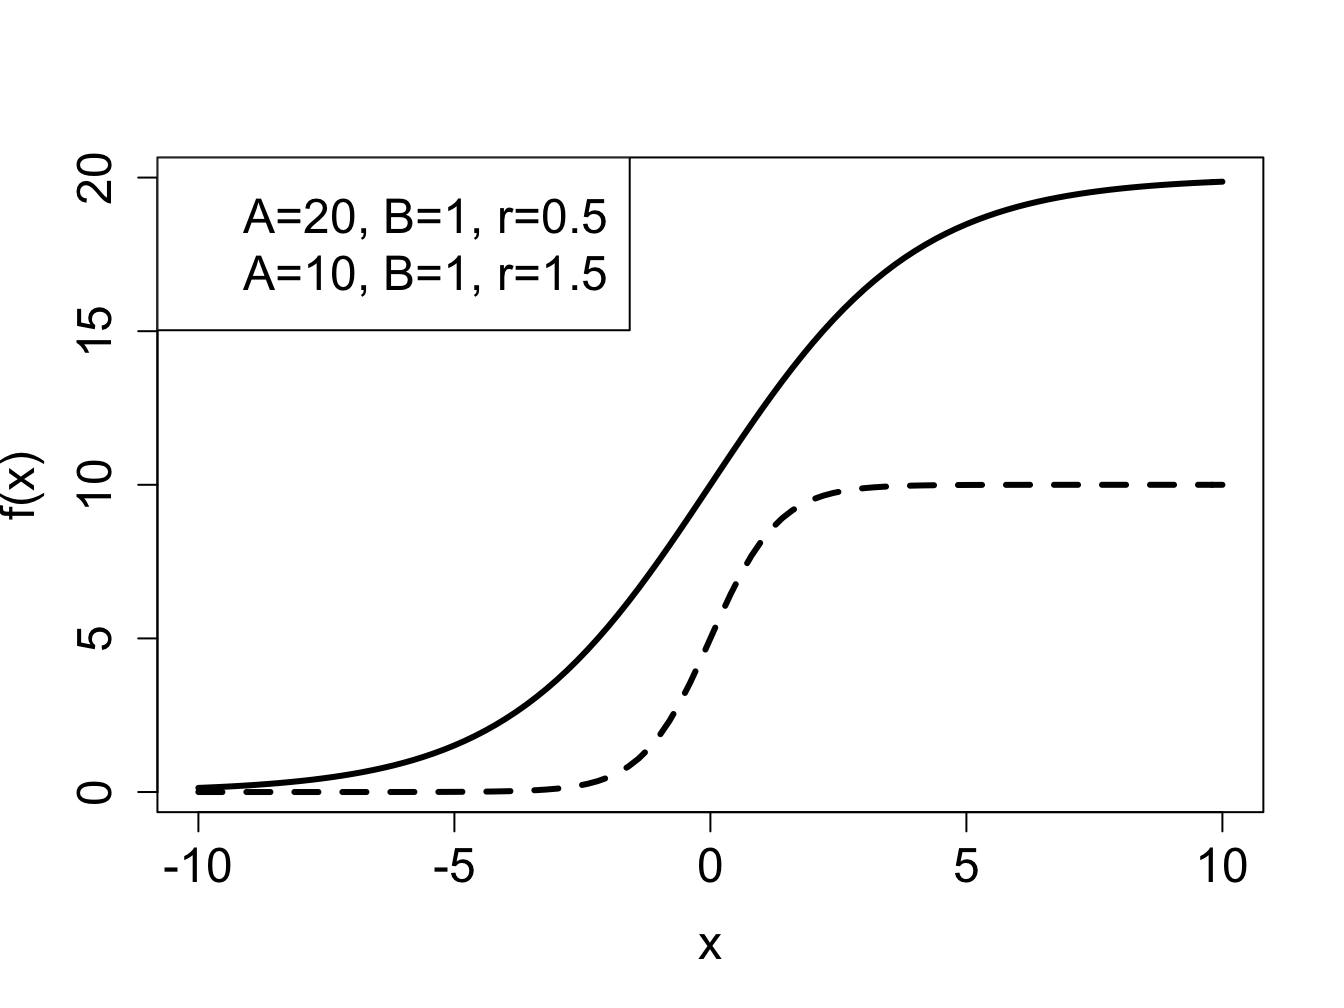
\includegraphics[width=0.5\linewidth]{QuantLife_files/figure-latex/ch2-funk2-1} 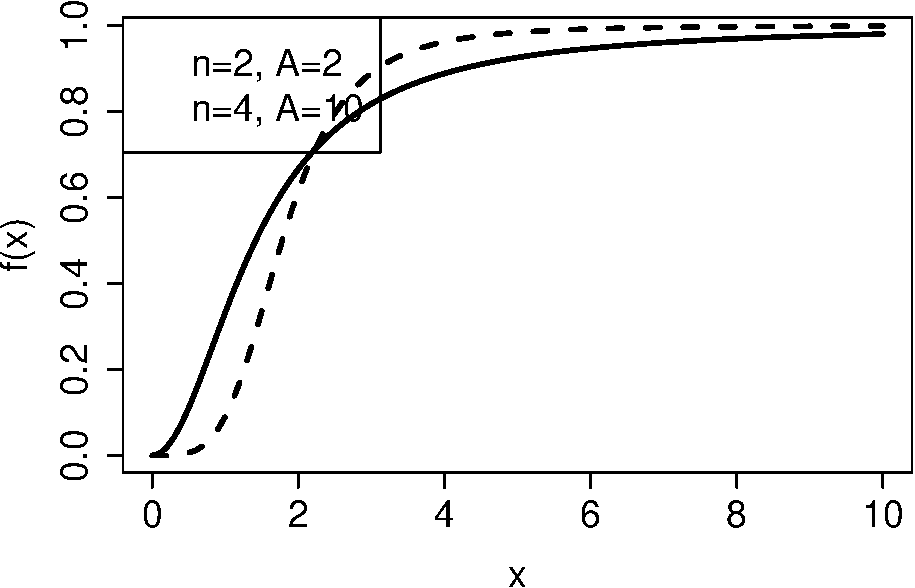
\includegraphics[width=0.5\linewidth]{QuantLife_files/figure-latex/ch2-funk2-2} 

}

\caption{Examples of two graphs of logistic functions (left) and two Hill functions (right).}\label{fig:ch2-funk2}
\end{figure}

\hypertarget{exercises-2}{%
\subsection{Exercises:}\label{exercises-2}}

For each biological model below answer the following questions in terms of the parameters in the models, assuming all are nonnegative real numbers. 1) what is the value of the function when the independent variable is 0? 2) what value does the function approach when the independent variable goes to infinity? 3) verbally describe the behavior of the functions between 0 and infinity (e.g., function increases, decreases).

\begin{enumerate}
\def\labelenumi{\arabic{enumi}.}
\item
  Model of number of mutations \(M\) as a function of time \(t\):
  \[ M(t) = M_0 + \mu t\]
\item
  Model of molecular concentration \(C\) as a function of time \(t\):
  \[ C(t) = C_0 e^{-kt} \]
\item
  Model of cooperative binding of ligands\index{model!binding cooperativity}, with fraction of bound receptors \(\theta\) as a function of ligand concentration \(L\):
  \[ \theta = \frac{L^n}{L^n + K_d}\]
\item
  Model of tree height \(H\) (length) as a function of age \(a\) (time):
  \[ H(a) = \frac{b a }{c + a}\]
\item
  Model of concentration of a gene product \(G\) (concentration) as a function of time \(t\):
  \[ G(t) = G_m (1 - e^{-\alpha t})\]
\item
  The simplified Goldman-Hodgkin-Katz model of ionic current \(I\) (current) as a function of membrane potential \(V\) (voltage):
  \[ I(V) = - b V \frac{1- c e^{-\alpha V}} {1-  e^{-\alpha V}} \]
\item
  Michaelis-Menten model \index{model!Michaelis-Menten} of enzyme kinetics, \(v\) is reaction rate (1/time) and \(S\) is substrate concentration:
  \[ v(S) = \frac{v_{max} S}{K_m + S}\]
\item
  Logistic model \index{logistic model}of population growth, \(P\) is population size and time \(t\):
  \[ P(t) = \frac{A e^{kt}}{1 + B(e^{kt} -1)} \]
\end{enumerate}

\hypertarget{vectors-and-plotting-in-r}{%
\section{Vectors and plotting in R}\label{vectors-and-plotting-in-r}}

\label{sec:comp2}

\hypertarget{writing-scripts-and-calling-functions}{%
\subsection{writing scripts and calling functions}\label{writing-scripts-and-calling-functions}}

Programming means arranging a number of commands in a particular order to perform a task. Typing them one at a time into the command line is inefficient and error-prone. Instead, the commands are written into a file called a program or script (the name depends on the type of language; since R is a scripting language you will be writing scripts), which can be edited, saved, copied, etc. To open a new script file, in R Studio, go to File menu, and choose New R Script. This will open an editor window where you can type your commands. To save the script file (do this often!!), click the Save button (with the little floppy disk icon) or select Save from the File menu. You will also see small buttons at the top of the window that say \texttt{Run}, \texttt{Re-run}, and \texttt{Source}. The first two will run either the current line or a selected region of the script, while the \texttt{Source} button will run the entire file. Now that you know how to create a script, \textbf{you should never type your R code into the command line}, unless you're testing a single command to see what it does, or looking up help.

R comes equipped with many \index{function!in R} \index{R programming!function} functions that correspond to standard mathematical functions. As we saw in section \ref{sec:comp1}, \texttt{exp()} is the exponential function that returns \(e\) raised to the power of the input value. Other common ones are: \texttt{sqrt()} returns the square root of the input value; \texttt{sin()} and \texttt{cos()} return the sine and the cosine of the input value, respectively. Note that all of these function names are followed by parentheses, which is a hallmark of a function (in R as well as in mathematics). This indicates that the input value has to go there, for example \texttt{exp(5)}. To compute the value of \(e^5\), save it into a variable called \texttt{var1} and then print out the value on the screen, you can create the following script:

\begin{Shaded}
\begin{Highlighting}[]
\NormalTok{var1 \textless{}{-}}\StringTok{ }\KeywordTok{exp}\NormalTok{(}\DecValTok{5}\NormalTok{)}
\KeywordTok{print}\NormalTok{(var1)}
\end{Highlighting}
\end{Shaded}

\begin{verbatim}
## [1] 148.4132
\end{verbatim}

If you run the above code chunk in R Studio you will see two things happen: a variable named var1 appears in the Environment window (top right) with the value 148.41\ldots{} and the same value is printed out in the command line window (bottom left).

The most important principle of the procedural brand of programming (which includes R) is this: the computer (that is, the compiler or interpreter) evaluates the commands from top to bottom, one at a time. The variables are used with the values that they are currently assigned. If one variable (\texttt{var1}) was assigned in terms of another (\texttt{var2}), and then \texttt{var2} is changed later, this does not change the value of \texttt{var2}. Here is an illustration of how this works:

\begin{Shaded}
\begin{Highlighting}[]
\NormalTok{var2 \textless{}{-}}\StringTok{ }\DecValTok{20}
\NormalTok{var1 \textless{}{-}}\StringTok{ }\NormalTok{var2}\OperatorTok{/}\DecValTok{20}
\KeywordTok{print}\NormalTok{(var2)}
\end{Highlighting}
\end{Shaded}

\begin{verbatim}
## [1] 20
\end{verbatim}

\begin{Shaded}
\begin{Highlighting}[]
\NormalTok{var2 \textless{}{-}}\StringTok{ }\DecValTok{10}
\KeywordTok{print}\NormalTok{(var1)}
\end{Highlighting}
\end{Shaded}

\begin{verbatim}
## [1] 1
\end{verbatim}

Notice that \texttt{var1} doesn't change, because the R interpreter reads the commands one by one, and does not go back to re-evaluate the assignment for var1 after \texttt{var2} is changed. Learning to think in this methodical, literal manner is crucial for developing programming skills.

\hypertarget{vector-variables}{%
\subsection{vector variables}\label{vector-variables}}

Variables may contain more than a single number, they can also store a bunch of numbers, which is then called an array. When numbers in an array are organized as a single ordered list, this is called a \index{R programming!vector variable}\index{vector!in R} \emph{vector}. There are several ways of producing a vector of numbers in R.

\hypertarget{c-function}{%
\subsubsection{c() function}\label{c-function}}

The most direct method of making a vector is to put together several values by listing them inside the function \texttt{c()} and assigning the output to a variable, e.g.~\texttt{my.vec}:

\begin{Shaded}
\begin{Highlighting}[]
\NormalTok{my.vec\textless{}{-}}\KeywordTok{c}\NormalTok{(pi,}\DecValTok{45}\NormalTok{,}\FloatTok{912.8}\NormalTok{, }\DecValTok{0}\NormalTok{)}
\KeywordTok{print}\NormalTok{(my.vec)}
\end{Highlighting}
\end{Shaded}

\begin{verbatim}
## [1]   3.141593  45.000000 912.800000   0.000000
\end{verbatim}

This variable \texttt{my.vec} is now a vector variable that contains four different numbers. Each of those numbers can be accessed individually by referencing its position in the vector, called the \index{R programming!index of vector} \emph{index}. In the R language the the index for the first number in a vector is 1, the index for the second number is 2, etc. The index is placed in square brackets after the vector name, as follows:

\begin{Shaded}
\begin{Highlighting}[]
\KeywordTok{print}\NormalTok{(my.vec[}\DecValTok{1}\NormalTok{])}
\end{Highlighting}
\end{Shaded}

\begin{verbatim}
## [1] 3.141593
\end{verbatim}

\begin{Shaded}
\begin{Highlighting}[]
\KeywordTok{print}\NormalTok{(my.vec[}\DecValTok{2}\NormalTok{])}
\end{Highlighting}
\end{Shaded}

\begin{verbatim}
## [1] 45
\end{verbatim}

\begin{Shaded}
\begin{Highlighting}[]
\KeywordTok{print}\NormalTok{(my.vec[}\DecValTok{3}\NormalTok{])}
\end{Highlighting}
\end{Shaded}

\begin{verbatim}
## [1] 912.8
\end{verbatim}

\begin{Shaded}
\begin{Highlighting}[]
\KeywordTok{print}\NormalTok{(my.vec[}\DecValTok{4}\NormalTok{])}
\end{Highlighting}
\end{Shaded}

\begin{verbatim}
## [1] 0
\end{verbatim}

\hypertarget{the-colon-operator}{%
\subsubsection{the colon operator}\label{the-colon-operator}}

Another way to generate a sequence of numbers in a particular order is to use the colon operator, which produces a vector of integers from the first number to the last, inclusive. Here are two examples:

\begin{Shaded}
\begin{Highlighting}[]
\NormalTok{my.vec1\textless{}{-}}\DecValTok{1}\OperatorTok{:}\DecValTok{20}
\KeywordTok{print}\NormalTok{(my.vec1)}
\end{Highlighting}
\end{Shaded}

\begin{verbatim}
##  [1]  1  2  3  4  5  6  7  8  9 10 11 12 13 14 15 16 17 18 19 20
\end{verbatim}

\begin{Shaded}
\begin{Highlighting}[]
\NormalTok{my.vec2\textless{}{-}}\DecValTok{0}\OperatorTok{:{-}}\DecValTok{20}
\KeywordTok{print}\NormalTok{(my.vec2)}
\end{Highlighting}
\end{Shaded}

\begin{verbatim}
##  [1]   0  -1  -2  -3  -4  -5  -6  -7  -8  -9 -10 -11 -12 -13 -14 -15 -16 -17 -18
## [20] -19 -20
\end{verbatim}

You can also access some but not all of the values stored in a vector simultaneously. To do this, enter a vector of positive integers inside the square brackets, either using the colon operator or using the \texttt{c()} function. Here are two examples, the first prints out the 4th through the 10th element of the vector \texttt{my.vec1}, while the second prints out the 1st, 5th, and 11th elements of the vector \texttt{my.vec2}:

\begin{Shaded}
\begin{Highlighting}[]
\KeywordTok{print}\NormalTok{(my.vec1[}\DecValTok{4}\OperatorTok{:}\DecValTok{10}\NormalTok{])}
\end{Highlighting}
\end{Shaded}

\begin{verbatim}
## [1]  4  5  6  7  8  9 10
\end{verbatim}

\begin{Shaded}
\begin{Highlighting}[]
\KeywordTok{print}\NormalTok{(my.vec2[}\KeywordTok{c}\NormalTok{(}\DecValTok{1}\NormalTok{,}\DecValTok{5}\NormalTok{,}\DecValTok{11}\NormalTok{)])}
\end{Highlighting}
\end{Shaded}

\begin{verbatim}
## [1]   0  -4 -10
\end{verbatim}

\hypertarget{seq-function}{%
\subsubsection{seq() function}\label{seq-function}}

If you want to generate a sequence of numbers with a constant difference other than 1, you're in luck: R provides a function called \texttt{seq()}. It takes three inputs: the starting value, the ending value, and the step (difference between successive elements). For example, to generate a list of numbers starting at 20 up to 50, with a step size of 3, type the first command; to obtain the same sequence in reverse, use the second command:

\begin{Shaded}
\begin{Highlighting}[]
\NormalTok{my.vec1\textless{}{-}}\KeywordTok{seq}\NormalTok{(}\DecValTok{20}\NormalTok{,}\DecValTok{50}\NormalTok{,}\DecValTok{3}\NormalTok{)}
\KeywordTok{print}\NormalTok{(my.vec1)}
\end{Highlighting}
\end{Shaded}

\begin{verbatim}
##  [1] 20 23 26 29 32 35 38 41 44 47 50
\end{verbatim}

\begin{Shaded}
\begin{Highlighting}[]
\NormalTok{my.vec2\textless{}{-}}\KeywordTok{seq}\NormalTok{(}\DecValTok{50}\NormalTok{,}\DecValTok{20}\NormalTok{,}\OperatorTok{{-}}\DecValTok{3}\NormalTok{)}
\KeywordTok{print}\NormalTok{(my.vec2)}
\end{Highlighting}
\end{Shaded}

\begin{verbatim}
##  [1] 50 47 44 41 38 35 32 29 26 23 20
\end{verbatim}

\hypertarget{rep-function}{%
\subsubsection{rep() function}\label{rep-function}}

Sometimes you want to create a vector of repeated values. For example, you can create a variable with 20 zeros, you can use rep() like this:

\begin{Shaded}
\begin{Highlighting}[]
\NormalTok{zeros \textless{}{-}}\StringTok{ }\KeywordTok{rep}\NormalTok{(}\DecValTok{0}\NormalTok{,}\DecValTok{20}\NormalTok{)}
\KeywordTok{print}\NormalTok{(zeros)}
\end{Highlighting}
\end{Shaded}

\begin{verbatim}
##  [1] 0 0 0 0 0 0 0 0 0 0 0 0 0 0 0 0 0 0 0 0
\end{verbatim}

You can repeat any value, say create a vector by repeating the number pi:

\begin{Shaded}
\begin{Highlighting}[]
\NormalTok{pies \textless{}{-}}\StringTok{ }\KeywordTok{rep}\NormalTok{(pi,}\DecValTok{7}\NormalTok{)}
\KeywordTok{print}\NormalTok{(pies)}
\end{Highlighting}
\end{Shaded}

\begin{verbatim}
## [1] 3.141593 3.141593 3.141593 3.141593 3.141593 3.141593 3.141593
\end{verbatim}

You can even repeat another vector, like the vector my.vec that was assigned above:

\begin{Shaded}
\begin{Highlighting}[]
\NormalTok{my.vecs \textless{}{-}}\StringTok{ }\KeywordTok{rep}\NormalTok{(my.vec, }\DecValTok{5}\NormalTok{)}
\KeywordTok{print}\NormalTok{(my.vecs)}
\end{Highlighting}
\end{Shaded}

\begin{verbatim}
##  [1]   3.141593  45.000000 912.800000   0.000000   3.141593  45.000000
##  [7] 912.800000   0.000000   3.141593  45.000000 912.800000   0.000000
## [13]   3.141593  45.000000 912.800000   0.000000   3.141593  45.000000
## [19] 912.800000   0.000000
\end{verbatim}

\hypertarget{calculations-with-vector-variables}{%
\subsection{calculations with vector variables}\label{calculations-with-vector-variables}}

\begin{Shaded}
\begin{Highlighting}[]
\NormalTok{NewVec \textless{}{-}}\StringTok{ }\DecValTok{2}\OperatorTok{*}\NormalTok{my.vec}
\KeywordTok{print}\NormalTok{(NewVec)}
\end{Highlighting}
\end{Shaded}

\begin{verbatim}
## [1]    6.283185   90.000000 1825.600000    0.000000
\end{verbatim}

You can also perform calculations with multiple vector variables, but this requires extra care. R can perform any arithmetic operation with two vector variables, for instance adding two vectors results in a vector containing the sum of corresponding elements of the two vectors:

\begin{Shaded}
\begin{Highlighting}[]
\NormalTok{my.vec1\textless{}{-}}\DecValTok{1}\OperatorTok{:}\DecValTok{5}
\NormalTok{my.vec2\textless{}{-}}\DecValTok{0}\OperatorTok{:}\DecValTok{4}
\KeywordTok{print}\NormalTok{(my.vec1)}
\end{Highlighting}
\end{Shaded}

\begin{verbatim}
## [1] 1 2 3 4 5
\end{verbatim}

\begin{Shaded}
\begin{Highlighting}[]
\KeywordTok{print}\NormalTok{(my.vec2)}
\end{Highlighting}
\end{Shaded}

\begin{verbatim}
## [1] 0 1 2 3 4
\end{verbatim}

\begin{Shaded}
\begin{Highlighting}[]
\NormalTok{sum.vec\textless{}{-}my.vec1}\OperatorTok{+}\NormalTok{my.vec2}
\KeywordTok{print}\NormalTok{(sum.vec)}
\end{Highlighting}
\end{Shaded}

\begin{verbatim}
## [1] 1 3 5 7 9
\end{verbatim}

One needs to take care that the two vectors have the same number of elements (length). If you try to operate on (e.g.~add) two vectors of different lengths, R will return a warning and the result will not be what you expect:

\begin{Shaded}
\begin{Highlighting}[]
\NormalTok{my.vec1\textless{}{-}}\DecValTok{1}\OperatorTok{:}\DecValTok{2}
\NormalTok{my.vec2\textless{}{-}}\DecValTok{0}\OperatorTok{:}\DecValTok{4}
\KeywordTok{print}\NormalTok{(my.vec1)}
\end{Highlighting}
\end{Shaded}

\begin{verbatim}
## [1] 1 2
\end{verbatim}

\begin{Shaded}
\begin{Highlighting}[]
\KeywordTok{print}\NormalTok{(my.vec2)}
\end{Highlighting}
\end{Shaded}

\begin{verbatim}
## [1] 0 1 2 3 4
\end{verbatim}

\begin{Shaded}
\begin{Highlighting}[]
\NormalTok{sum.vec\textless{}{-}my.vec1}\OperatorTok{+}\NormalTok{my.vec2}
\end{Highlighting}
\end{Shaded}

\begin{verbatim}
## Warning in my.vec1 + my.vec2: longer object length is not a multiple of shorter
## object length
\end{verbatim}

\begin{Shaded}
\begin{Highlighting}[]
\KeywordTok{print}\NormalTok{(sum.vec)}
\end{Highlighting}
\end{Shaded}

\begin{verbatim}
## [1] 1 3 3 5 5
\end{verbatim}

\hypertarget{exercises-3}{%
\subsection{Exercises}\label{exercises-3}}

The following R commands or short scripts contain errors; your job is to fix them so they runs as described.

\begin{enumerate}
\def\labelenumi{\arabic{enumi}.}
\tightlist
\item
  Assign a vector of three numbers to a variable:
\end{enumerate}

\begin{Shaded}
\begin{Highlighting}[]
\NormalTok{date\_num \textless{}{-}}\StringTok{ }\NormalTok{(}\DecValTok{3}\NormalTok{,}\DecValTok{8}\NormalTok{,}\DecValTok{16}\NormalTok{)}
\end{Highlighting}
\end{Shaded}

\begin{enumerate}
\def\labelenumi{\arabic{enumi}.}
\setcounter{enumi}{1}
\tightlist
\item
  Assign a range of values to a vector variable and print out the third one:
\end{enumerate}

\begin{Shaded}
\begin{Highlighting}[]
\NormalTok{the.vals \textless{}{-}}\StringTok{ }\DecValTok{0}\OperatorTok{:}\DecValTok{10}
\NormalTok{print[}\KeywordTok{the.vals}\NormalTok{(}\DecValTok{3}\NormalTok{)]}
\end{Highlighting}
\end{Shaded}

\begin{enumerate}
\def\labelenumi{\arabic{enumi}.}
\setcounter{enumi}{2}
\tightlist
\item
  Assign a range of values to a vector variable and print out the fourtieth and sixty-first values:
\end{enumerate}

\begin{Shaded}
\begin{Highlighting}[]
\NormalTok{all.the.vals \textless{}{-}}\StringTok{ }\DecValTok{0}\OperatorTok{:}\DecValTok{100}
\KeywordTok{print}\NormalTok{(all.the.vals[}\DecValTok{40}\NormalTok{,}\DecValTok{61}\NormalTok{])}
\end{Highlighting}
\end{Shaded}

\begin{enumerate}
\def\labelenumi{\arabic{enumi}.}
\setcounter{enumi}{3}
\tightlist
\item
  Take the two vectors assigned above and assign their product to another vector:
\end{enumerate}

\begin{Shaded}
\begin{Highlighting}[]
\NormalTok{product \textless{}{-}}\StringTok{ }\NormalTok{the.vals}\OperatorTok{*}\NormalTok{all.the.vals}
\end{Highlighting}
\end{Shaded}

\begin{enumerate}
\def\labelenumi{\arabic{enumi}.}
\setcounter{enumi}{4}
\tightlist
\item
  Create a vector vec1 of ten integers and print the second and the eighth elements:
\end{enumerate}

\begin{Shaded}
\begin{Highlighting}[]
\NormalTok{vec1 \textless{}{-}}\StringTok{ }\DecValTok{11}\OperatorTok{:}\DecValTok{20} 
\KeywordTok{print}\NormalTok{(vec1[}\DecValTok{2}\OperatorTok{:}\DecValTok{8}\NormalTok{])}
\end{Highlighting}
\end{Shaded}

\begin{enumerate}
\def\labelenumi{\arabic{enumi}.}
\setcounter{enumi}{5}
\tightlist
\item
  Create a vector \texttt{vec1} and then multiply all of its elements by 20 and assign it to another vector:
\end{enumerate}

\begin{Shaded}
\begin{Highlighting}[]
\NormalTok{vec1\textless{}{-}}\KeywordTok{seq}\NormalTok{(}\OperatorTok{{-}}\DecValTok{3}\NormalTok{,}\DecValTok{2}\NormalTok{,}\FloatTok{0.1}\NormalTok{)}
\NormalTok{vec2 \textless{}{-}}\StringTok{ }\NormalTok{20vec1}
\end{Highlighting}
\end{Shaded}

\begin{enumerate}
\def\labelenumi{\arabic{enumi}.}
\setcounter{enumi}{6}
\tightlist
\item
  Create a vector \texttt{vec1}, a vector \texttt{vec2} and print out all the elements of the first divided by the second:
\end{enumerate}

\begin{Shaded}
\begin{Highlighting}[]
\NormalTok{vec1 \textless{}{-}}\StringTok{ }\DecValTok{0}\OperatorTok{:}\DecValTok{5}
\NormalTok{vec2 \textless{}{-}}\StringTok{ }\DecValTok{3}\OperatorTok{:}\DecValTok{8}
\NormalTok{print[vec1}\OperatorTok{/}\NormalTok{vec2]}
\end{Highlighting}
\end{Shaded}

\hypertarget{plotting-with-vectors}{%
\subsection{Plotting with vectors}\label{plotting-with-vectors}}

\begin{Shaded}
\begin{Highlighting}[]
\KeywordTok{curve}\NormalTok{(x}\OperatorTok{\^{}}\DecValTok{2}\NormalTok{,}\DecValTok{0}\NormalTok{,}\DecValTok{10}\NormalTok{,}\DataTypeTok{lwd=}\DecValTok{3}\NormalTok{,}\DataTypeTok{xlab=}\StringTok{\textquotesingle{}x\textquotesingle{}}\NormalTok{, }\DataTypeTok{ylab=}\StringTok{\textquotesingle{}quadratic\textquotesingle{}}\NormalTok{,}\DataTypeTok{cex.axis=}\FloatTok{1.5}\NormalTok{,}\DataTypeTok{cex.lab=}\FloatTok{1.5}\NormalTok{)}
\KeywordTok{curve}\NormalTok{(}\DecValTok{20}\OperatorTok{*}\KeywordTok{exp}\NormalTok{(}\OperatorTok{{-}}\FloatTok{0.5}\OperatorTok{*}\NormalTok{x),}\DecValTok{0}\NormalTok{,}\DecValTok{5}\NormalTok{,}\DataTypeTok{lwd=}\DecValTok{3}\NormalTok{,}\DataTypeTok{xlab=}\StringTok{\textquotesingle{}x\textquotesingle{}}\NormalTok{, }\DataTypeTok{ylab=}\StringTok{\textquotesingle{}exponential\textquotesingle{}}\NormalTok{,}\DataTypeTok{cex.axis=}\FloatTok{1.5}\NormalTok{,}\DataTypeTok{cex.lab=}\FloatTok{1.5}\NormalTok{)}
\end{Highlighting}
\end{Shaded}

\begin{figure}

{\centering 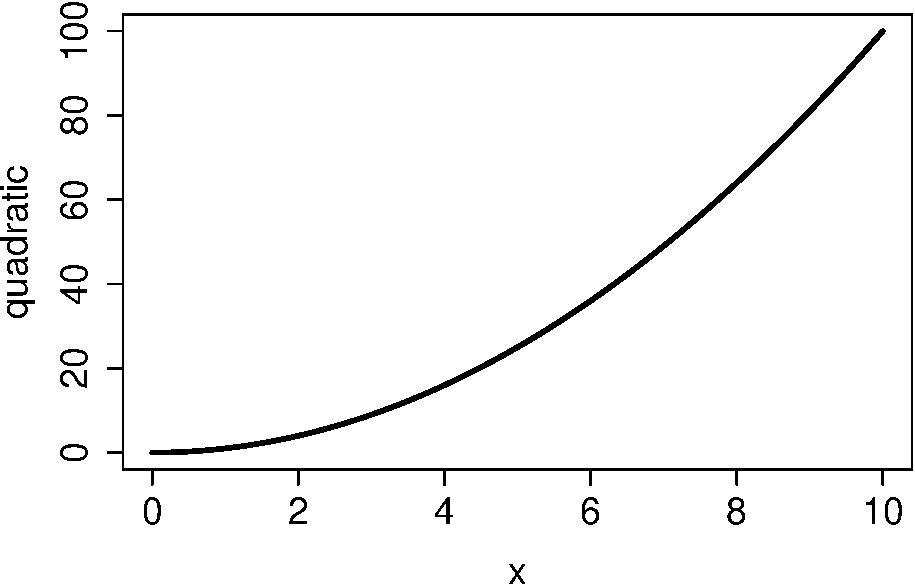
\includegraphics[width=0.5\linewidth]{QuantLife_files/figure-latex/ch2-plot1-1} 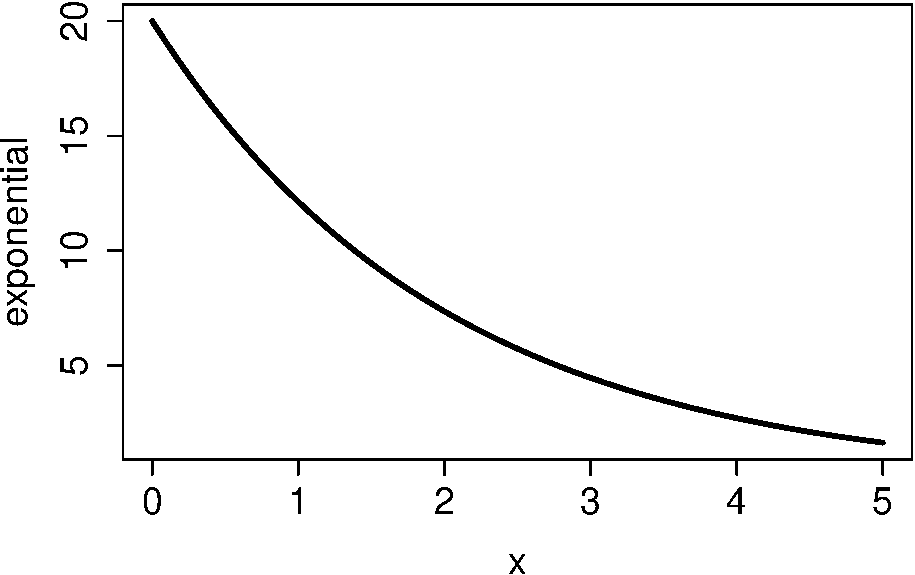
\includegraphics[width=0.5\linewidth]{QuantLife_files/figure-latex/ch2-plot1-2} 

}

\caption{Two examples of plots using curve: quadratic ($y=x^2$) and exponential ($y=20*e^{-0.5x}$)}\label{fig:ch2-plot1}
\end{figure}

There are several ways of \index{plot!in R} \index{R programming!plotting} creating plots of mathematical functions or data R. If you want to plot a mathematical function, the simplest function is \texttt{curve()}. You can tell that this is a function, because it uses parentheses; the first input is an expression for the function, and the next two define the range of the independent variable over which to plot the graph. Two examples of plotting a quadratic function over the range from 0 and 5, and an exponential variation over the range of 0 to 10 are shown in figure \ref{fig:ch2-plot1}.

One can change the default look of the plot produced by curve by setting different options, which are optional inputs into the curve function, One is the line width \texttt{lwd} which can be increased from the default value of 1 to produce thicker curves, as demonstrated in the example above. One can add labels on the x and y axes with \texttt{xlab} and \texttt{ylab} options, respectively; note that these are strings of characters, and thus must be put in quotes to differentiate them from a variable name. There is one very important option not shown above: that of overlaying a curve on top of an existing plot, which is done by typing \texttt{add=TRUE}. This option takes logical (Boolean) values \texttt{TRUE} and \texttt{FALSE}, which must be typed in all caps and without quotes.

\hypertarget{plot-function}{%
\subsubsection{plot() function}\label{plot-function}}

In addition to curve, one can use the function \texttt{plot()} in R to create two dimensional graphs from two vector-valued variables of the same length, e.g.~\texttt{plot(x,y)}. The first input variable corresponds to the \index{variable!independent} \emph{independent variable} (e.g.~\texttt{x}), which is plotted on the x-axis, and the second variable corresponds to the \index{variable!dependent} \emph{dependent variable} (e.g.~\texttt{y}) which is plotted on the y-axis. In figure \ref{fig:ch2-plot2} you see graphs of exponential and logistic function plotted using \texttt{plot()}.

The following chunk creates a vector variable time, then calculates a new variable quad using time in a single operation:

\begin{Shaded}
\begin{Highlighting}[]
\NormalTok{time \textless{}{-}}\StringTok{ }\DecValTok{0}\OperatorTok{:}\DecValTok{10}
\NormalTok{quad \textless{}{-}}\StringTok{ }\NormalTok{(time }\OperatorTok{{-}}\StringTok{ }\DecValTok{5}\NormalTok{)}\OperatorTok{\^{}}\DecValTok{2}
\KeywordTok{print}\NormalTok{(time)}
\end{Highlighting}
\end{Shaded}

\begin{verbatim}
##  [1]  0  1  2  3  4  5  6  7  8  9 10
\end{verbatim}

\begin{Shaded}
\begin{Highlighting}[]
\KeywordTok{print}\NormalTok{(quad)}
\end{Highlighting}
\end{Shaded}

\begin{verbatim}
##  [1] 25 16  9  4  1  0  1  4  9 16 25
\end{verbatim}

This chunk plots the two vector variables quad as a function of time, and adds a title to the plot

\begin{Shaded}
\begin{Highlighting}[]
\KeywordTok{plot}\NormalTok{(time,quad, }\DataTypeTok{main =} \StringTok{\textquotesingle{}Quadratic function of time\textquotesingle{}}\NormalTok{)}
\end{Highlighting}
\end{Shaded}

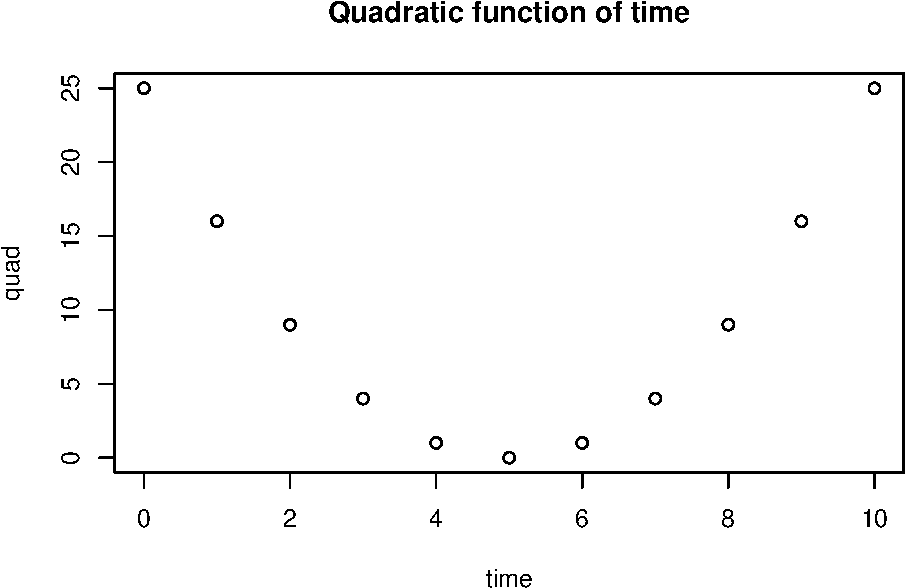
\includegraphics{QuantLife_files/figure-latex/unnamed-chunk-41-1.pdf}

The default plot style in R uses circles to indicate each plotted point. To change it, you need to set the option \texttt{t} (type), for example, setting \texttt{t=\textquotesingle{}l\textquotesingle{}} (the lowercase letter L) produces a continuous line connecting the individual data points.

\begin{Shaded}
\begin{Highlighting}[]
\KeywordTok{plot}\NormalTok{(time,quad, }\DataTypeTok{main =} \StringTok{\textquotesingle{}Quadratic function of time\textquotesingle{}}\NormalTok{, }\DataTypeTok{type =} \StringTok{\textquotesingle{}l\textquotesingle{}}\NormalTok{, }\DataTypeTok{xlab=}\StringTok{\textquotesingle{}time\textquotesingle{}}\NormalTok{, }\DataTypeTok{ylab =} \StringTok{\textquotesingle{}y = f(t)\textquotesingle{}}\NormalTok{ )}
\end{Highlighting}
\end{Shaded}

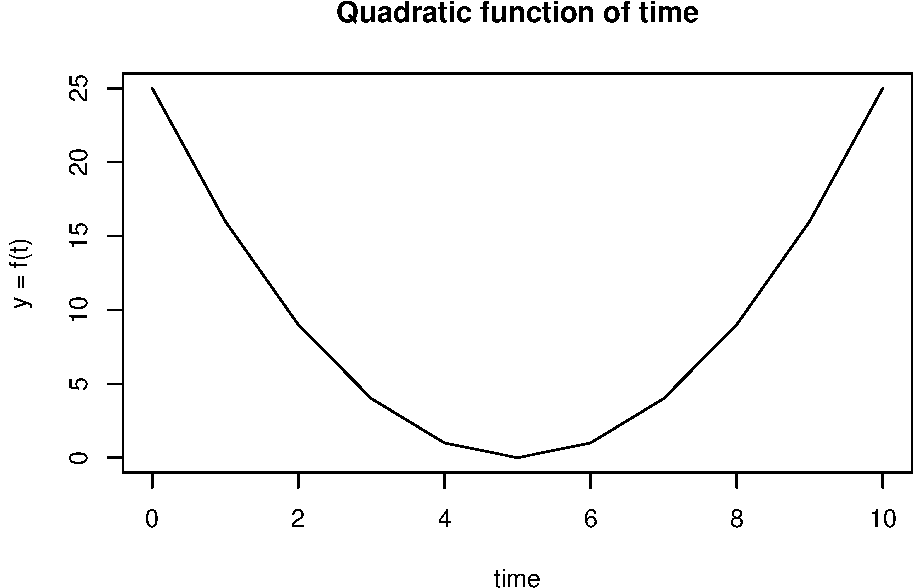
\includegraphics{QuantLife_files/figure-latex/unnamed-chunk-42-1.pdf}

\texttt{plot()} is a versatile function that has many options function has many options which can be changed to determine the color, the style, and other attributes of the plot. For a full list type \texttt{help(plot)} in the console or type plot in the search bar of the Help pane in the bottom right window.

\hypertarget{using-lines-or-points}{%
\subsubsection{using lines() or points()}\label{using-lines-or-points}}

You may also want to plot multiple graphs on the same figure. The \texttt{plot()} function creates a new plot window, so if you want to add another plot on top of the first one, you have to use another function. There are two ones available: \texttt{lines()} which produces continuous curves connecting the points, and \texttt{points()} which plots individual symbols at every point.

Let us illustrate this by plotting two different exponential functions on one plot, and two different logistic functions on the second one, which were discussed in section \ref{sec:math2}. When you've got multiple plots on the same figure, they need to be distinct and labeled. To distinguish them, below I use the option \texttt{col} to specify the color of the plot, and I add a legend describing the parameters of each plot to the figure \ref{fig:ch2-plot2}. The function has a lot of options, so if you want to understand the details, type \texttt{help(legend)} in the prompt or go to Help tab in the lower right frame of R Studio and type legend.

\begin{Shaded}
\begin{Highlighting}[]
\NormalTok{x\textless{}{-}}\KeywordTok{seq}\NormalTok{(}\DecValTok{0}\NormalTok{,}\DecValTok{10}\NormalTok{,}\FloatTok{0.5}\NormalTok{)}
\NormalTok{y\textless{}{-}}\DecValTok{10}\OperatorTok{+}\DecValTok{20}\OperatorTok{*}\KeywordTok{exp}\NormalTok{(}\OperatorTok{{-}}\FloatTok{0.5}\OperatorTok{*}\NormalTok{x)}
\KeywordTok{plot}\NormalTok{(x,y, }\DataTypeTok{xlab=}\StringTok{\textquotesingle{}x\textquotesingle{}}\NormalTok{, }\DataTypeTok{ylab=}\StringTok{\textquotesingle{}exponential\textquotesingle{}}\NormalTok{,}\DataTypeTok{col=}\DecValTok{1}\NormalTok{,}\DataTypeTok{lwd=}\DecValTok{3}\NormalTok{)}
\NormalTok{y\textless{}{-}}\DecValTok{10}\OperatorTok{+}\DecValTok{20}\OperatorTok{*}\KeywordTok{exp}\NormalTok{(}\OperatorTok{{-}}\DecValTok{2}\OperatorTok{*}\NormalTok{x)}
\KeywordTok{lines}\NormalTok{(x,y,}\DataTypeTok{col=}\DecValTok{2}\NormalTok{,}\DataTypeTok{lwd=}\DecValTok{3}\NormalTok{)}
\NormalTok{leg.txt=}\KeywordTok{c}\NormalTok{(}\StringTok{"b=10,a=20,r={-}0.5"}\NormalTok{, }\StringTok{"b=10,a=20,r={-}2"}\NormalTok{)}
\KeywordTok{legend}\NormalTok{(}\StringTok{"topright"}\NormalTok{, leg.txt, }\DataTypeTok{col=}\DecValTok{1}\OperatorTok{:}\DecValTok{2}\NormalTok{, }\DataTypeTok{pch=}\KeywordTok{c}\NormalTok{(}\DecValTok{1}\NormalTok{,}\OtherTok{NA}\NormalTok{), }\DataTypeTok{lty=}\KeywordTok{c}\NormalTok{(}\DecValTok{0}\NormalTok{,}\DecValTok{1}\NormalTok{), }\DataTypeTok{lwd=}\DecValTok{3}\NormalTok{)}
\NormalTok{x\textless{}{-}}\KeywordTok{seq}\NormalTok{(}\OperatorTok{{-}}\DecValTok{10}\NormalTok{,}\DecValTok{10}\NormalTok{,}\DecValTok{1}\NormalTok{)}
\NormalTok{y\textless{}{-}}\DecValTok{20}\OperatorTok{*}\KeywordTok{exp}\NormalTok{(}\FloatTok{0.5}\OperatorTok{*}\NormalTok{x)}\OperatorTok{/}\NormalTok{(}\DecValTok{1}\OperatorTok{+}\KeywordTok{exp}\NormalTok{(}\FloatTok{0.5}\OperatorTok{*}\NormalTok{x))}
\KeywordTok{plot}\NormalTok{(x,y,}\DataTypeTok{xlab=}\StringTok{\textquotesingle{}x\textquotesingle{}}\NormalTok{,}\DataTypeTok{ylab=}\StringTok{\textquotesingle{}logistic\textquotesingle{}}\NormalTok{,}\DataTypeTok{col=}\DecValTok{4}\NormalTok{,}\DataTypeTok{lwd=}\DecValTok{3}\NormalTok{)}
\NormalTok{y\textless{}{-}}\DecValTok{20}\OperatorTok{*}\KeywordTok{exp}\NormalTok{(}\FloatTok{1.5}\OperatorTok{*}\NormalTok{x)}\OperatorTok{/}\NormalTok{(}\DecValTok{1}\OperatorTok{+}\KeywordTok{exp}\NormalTok{(}\FloatTok{1.5}\OperatorTok{*}\NormalTok{x))}
\KeywordTok{lines}\NormalTok{(x,y,}\DataTypeTok{col=}\DecValTok{2}\NormalTok{,}\DataTypeTok{lwd=}\DecValTok{3}\NormalTok{)}
\NormalTok{leg.txt=}\KeywordTok{c}\NormalTok{(}\StringTok{"a=20,b=1,r=0.5"}\NormalTok{, }\StringTok{"a=20,b=1,r=1.5"}\NormalTok{)}
\KeywordTok{legend}\NormalTok{(}\StringTok{"topleft"}\NormalTok{, leg.txt, }\DataTypeTok{col=}\KeywordTok{c}\NormalTok{(}\DecValTok{4}\NormalTok{,}\DecValTok{2}\NormalTok{), }\DataTypeTok{pch=}\KeywordTok{c}\NormalTok{(}\DecValTok{1}\NormalTok{,}\OtherTok{NA}\NormalTok{), }\DataTypeTok{lty=}\KeywordTok{c}\NormalTok{(}\DecValTok{0}\NormalTok{,}\DecValTok{1}\NormalTok{), }\DataTypeTok{lwd=}\DecValTok{3}\NormalTok{)}
\end{Highlighting}
\end{Shaded}

\begin{figure}

{\centering 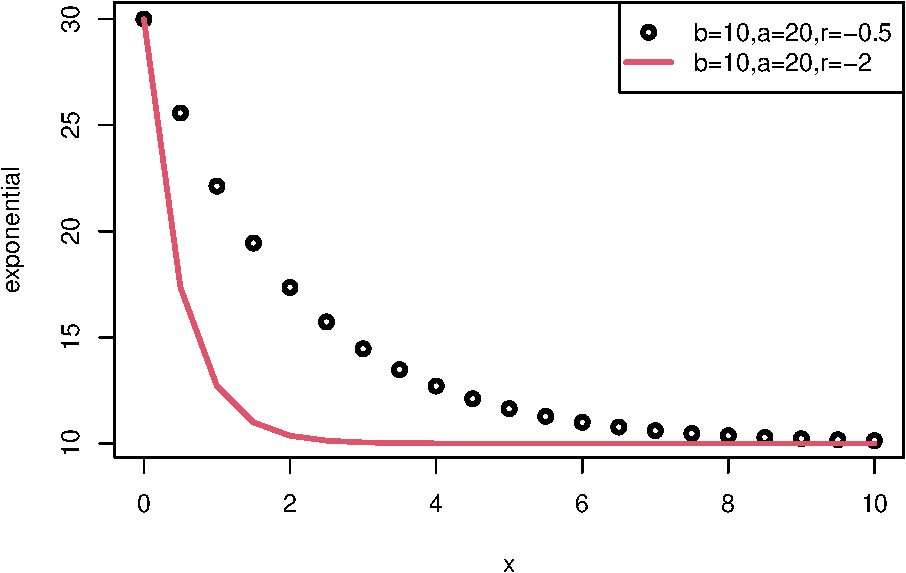
\includegraphics[width=0.5\linewidth]{QuantLife_files/figure-latex/ch2-plot2-1} 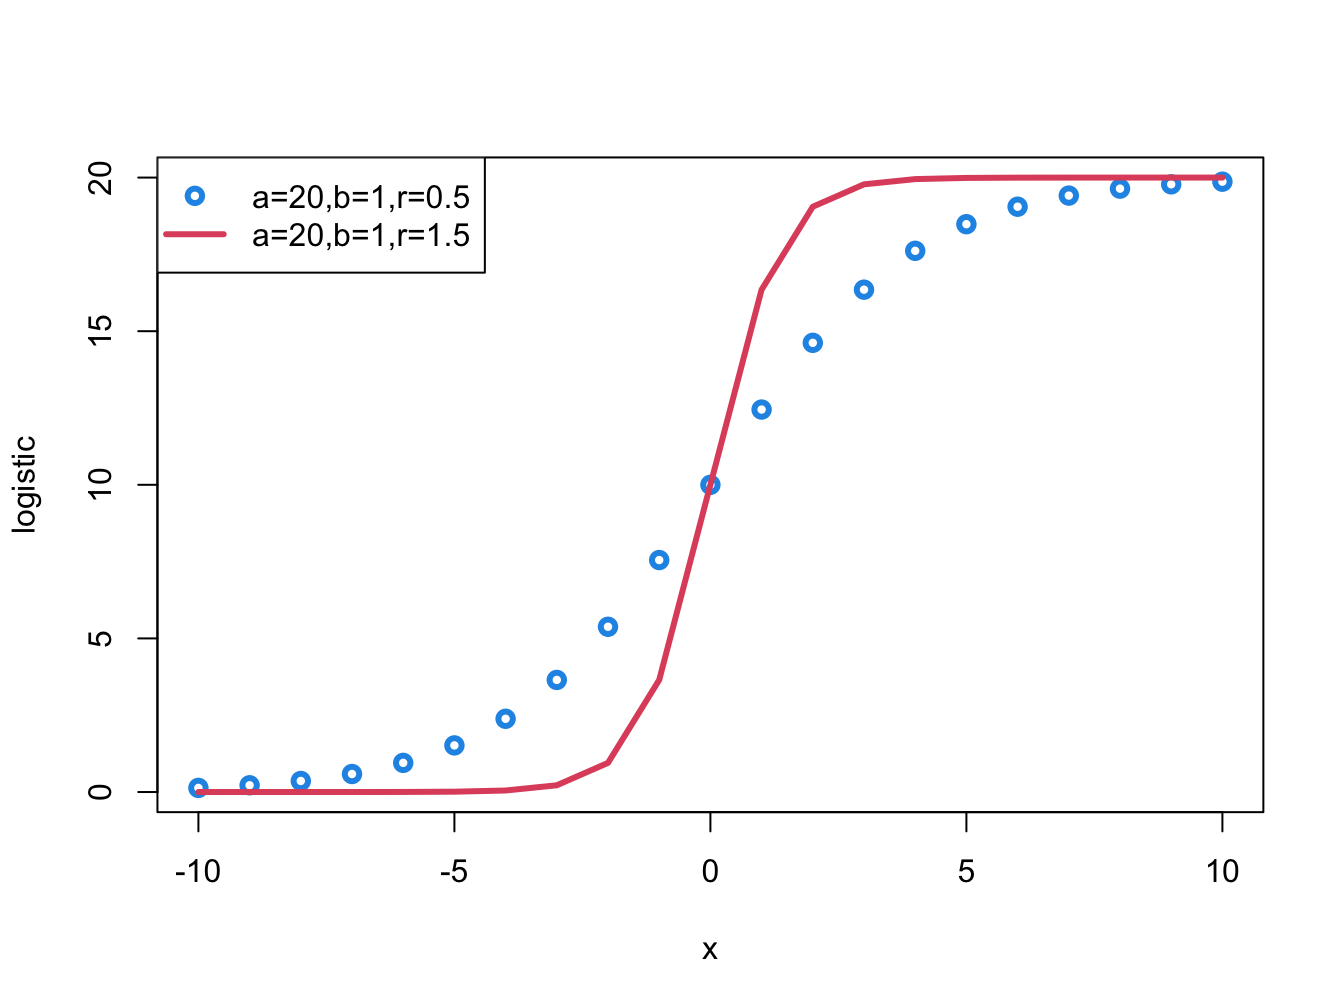
\includegraphics[width=0.5\linewidth]{QuantLife_files/figure-latex/ch2-plot2-2} 

}

\caption{Overlaying multiple plots in R: two exponential functions of the form $y=b+ae^{rx}$ on the left, two logistic functions of the form $y= ae^{rx}/(b+e^{rx})$ on the right.}\label{fig:ch2-plot2}
\end{figure}

\hypertarget{exercises-4}{%
\subsection{Exercises}\label{exercises-4}}

The following R commands or short scripts contain errors; your job is to fix them so they runs as described.

\begin{enumerate}
\def\labelenumi{\arabic{enumi}.}
\tightlist
\item
  Multiply a vector by a constant and add another constant and assign the result to a vector:
\end{enumerate}

\begin{Shaded}
\begin{Highlighting}[]
\NormalTok{new.vals \textless{}{-}}\StringTok{ }\DecValTok{5} \OperatorTok{+}\StringTok{ }\NormalTok{8the.vals}
\end{Highlighting}
\end{Shaded}

\begin{enumerate}
\def\labelenumi{\arabic{enumi}.}
\setcounter{enumi}{1}
\tightlist
\item
  Assign range to be a sequence of values from 0 to 100 with step of 0.1, and calculate the vector variable result as the square of the vector variable range:
\end{enumerate}

\begin{Shaded}
\begin{Highlighting}[]
\NormalTok{range \textless{}{-}}\StringTok{ }\KeywordTok{seq}\NormalTok{(}\DecValTok{0}\NormalTok{,}\FloatTok{0.1}\NormalTok{,}\DecValTok{100}\NormalTok{)}
\NormalTok{result \textless{}{-}}\StringTok{ }\KeywordTok{square}\NormalTok{(range)}
\end{Highlighting}
\end{Shaded}

\begin{enumerate}
\def\labelenumi{\arabic{enumi}.}
\setcounter{enumi}{2}
\tightlist
\item
  Plot result as a function of range:
\end{enumerate}

\begin{Shaded}
\begin{Highlighting}[]
\KeywordTok{plot}\NormalTok{(result, range)}
\end{Highlighting}
\end{Shaded}

\begin{enumerate}
\def\labelenumi{\arabic{enumi}.}
\setcounter{enumi}{3}
\tightlist
\item
  Plot the graph of the function \(f(x) = (45-x)/(4x+3)\) over the range of 0 to 100:
\end{enumerate}

\begin{Shaded}
\begin{Highlighting}[]
\KeywordTok{curve}\NormalTok{((}\DecValTok{45}\OperatorTok{{-}}\NormalTok{x)}\OperatorTok{/}\NormalTok{(4x}\OperatorTok{+}\DecValTok{3}\NormalTok{), }\DecValTok{0}\NormalTok{, }\DecValTok{100}\NormalTok{)}
\end{Highlighting}
\end{Shaded}

\begin{enumerate}
\def\labelenumi{\arabic{enumi}.}
\setcounter{enumi}{4}
\tightlist
\item
  Plot a quadratic function with specified coefficients \(a\), \(b\), \(c\) over a given range of independent variable \(x\):
\end{enumerate}

\begin{Shaded}
\begin{Highlighting}[]
\NormalTok{a\textless{}{-}}\DecValTok{10}
\NormalTok{b\textless{}{-}}\StringTok{ }\DecValTok{{-}15}
\NormalTok{c\textless{}{-}}\StringTok{ }\DecValTok{5}
\NormalTok{y\textless{}{-}a}\OperatorTok{*}\NormalTok{x}\OperatorTok{\^{}}\DecValTok{2}\OperatorTok{+}\NormalTok{b}\OperatorTok{*}\NormalTok{x}\OperatorTok{+}\NormalTok{c}
\NormalTok{x\textless{}{-}}\KeywordTok{seq}\NormalTok{(}\OperatorTok{{-}}\FloatTok{0.5}\NormalTok{,}\DecValTok{2}\NormalTok{,}\FloatTok{0.01}\NormalTok{) }
\KeywordTok{plot}\NormalTok{(x,y,}\DataTypeTok{type=}\StringTok{\textquotesingle{}l\textquotesingle{}}\NormalTok{)}
\end{Highlighting}
\end{Shaded}

\begin{enumerate}
\def\labelenumi{\arabic{enumi}.}
\setcounter{enumi}{5}
\tightlist
\item
  Overlay two different plots of the logistic function with different values of the parameter \(r\):
\end{enumerate}

\begin{Shaded}
\begin{Highlighting}[]
\NormalTok{time\textless{}{-}}\DecValTok{0}\OperatorTok{:}\DecValTok{100}
\NormalTok{a\textless{}{-}}\DecValTok{1000}
\NormalTok{b\textless{}{-}}\DecValTok{50} 
\NormalTok{r\textless{}{-}}\FloatTok{0.1}
\NormalTok{Population\textless{}{-}a}\OperatorTok{*}\KeywordTok{exp}\NormalTok{(r}\OperatorTok{*}\NormalTok{time)}\OperatorTok{/}\NormalTok{(b}\OperatorTok{+}\KeywordTok{exp}\NormalTok{(r}\OperatorTok{*}\NormalTok{time)) }
\KeywordTok{plot}\NormalTok{(time,Population,}\DataTypeTok{type=}\StringTok{\textquotesingle{}l\textquotesingle{}}\NormalTok{) }
\NormalTok{r\textless{}{-}}\DecValTok{10} 
\KeywordTok{lines}\NormalTok{(time,Population,}\DataTypeTok{col=}\DecValTok{2}\NormalTok{)}
\end{Highlighting}
\end{Shaded}

\hypertarget{rates-of-biochemical-reactions}{%
\section{Rates of biochemical reactions\}}\label{rates-of-biochemical-reactions}}

\label{sec:bio2}

Living things are dynamic, they change with time, and much of mathematical modeling in biology is interested in describing these changes. Some quantities change fast and others slowly, and every dynamic quantity has a rate of change, or \emph{rate} for short. Usually, the quantity that we want to track over time is the variable, and in order to describe how it changes we introduce a rate parameter. If we are describing changes over time, all rate parameters have dimensions with time in the denominator. As a simple example, the velocity of a physical object describes the change in distance over time, so its dimension is \([v] = length/time\).

Molecular reactions are essential for biology, whether they happen inside a bacterial cell or in the bloodstream of a human. \emph{Reaction kinetics} \index{kinetics!reaction} refers to the description of the rates, or the speed, of chemical reactions. Different reactions occur with different rates, which may be dependent on the concentration of the reactant molecule. Consider a simple reaction of molecule \(A\) turning into molecule \(B\), which is usually written by chemists with an arrow:
\[
  A \xrightarrow{k} B
\]
But how fast does the reaction take place? To write down a mathematical model, we need to define the quantities involved. First, we have the concentration of the molecule \(A\), with dimensions of concentration. Second, we have the rate of reaction, let us call it \(v\), which has dimension of concentration per time (just like velocity is length per time). How are the two quantities related?

\hypertarget{constant-zeroth-order-kinetics}{%
\subsection{Constant (zeroth-order) kinetics}\label{constant-zeroth-order-kinetics}}

\index{kinetics!zeroth-order} In some circumstances, the reaction rate \(v\) does not depend on the concentration of the reactant molecule \(A\). In that case, the relationship between the \index{kinetics!rate constant} \emph{rate constant} \(k\) and the actual rate \(v\) is:
\begin{equation}
v = k
\label{eq:kinetics_0th_order}
\end{equation}

Dimensional analysis insists that the dimension of \(k\) must be the dimension of \(v\), or concentration/time. This is known as constant, or zero-order kinetics, and it is observed at concentrations of \(A\) when the reaction is at its maximum velocity: for example, ethanol metabolism by ethanol dehydrogenase in human liver cannot proceed any faster than about 1 drink per hour.

\hypertarget{first-order-kinetics}{%
\subsection{First-order kinetics}\label{first-order-kinetics}}

\index{kinetics!first-order}. In other conditions, it is easy to imagine that increasing the concentration of the reactant \(A\) will speed up the rate of the reaction. A simple relationship of this type is linear:
\begin{equation}
v = kA
\label{eq:kinetics_1st_order}
\end{equation}

In this case, the dimension of the rate constant \(k\) is 1/time. This is called first-order kinetics, and it usually describes reactions when the concentration of \(A\) is small, and there are plenty of free enzymes to catalyze more reactions.

\hypertarget{michaelis-menten-model-of-enzyme-kinetics}{%
\subsection{\texorpdfstring{Michaelis-Menten model of enzyme kinetics \index{kinetics!Michaelis-Menten}}{Michaelis-Menten model of enzyme kinetics }}\label{michaelis-menten-model-of-enzyme-kinetics}}

However, if the concentration of the molecule is neither small nor large, we need to consider a more sophisticated model. An enzyme is a protein which catalyzes a biochemical reaction, and it works in two steps: first it binds the substrate, at which point it can still dissociate and float away, and then it actually catalyzes the reaction, which is usually practically irreversible (at least by this enzyme) and releases the product. The enzyme itself is not affected or spent, so it is free to catalyze more reactions. Let denote the substrate (reactant) molecule by \(A\), the product molecule by \(B\), the enzyme by \(E\), and the complex of substrate and enzyme \(AE\). The classic chemical scheme that describes these reactions is this:
\[
A + E \xrightleftharpoons[k_{-1}]{k_1} AE  \xrightarrow{k_2} E + B
\]

You could write three different kinetic equations for the three different arrows in that scheme. Michaelis and Menten used the simplifying assumptions that the binding and dissociation happens much faster than the catalytic reaction, and based on this they were able to write down an approximate, but extremely useful Michaelis-Menten model of an enzymatic reaction:
\begin{equation}
v = \frac{v_{max} A}{K_M+A}
\label{eq:kinetics_MM_kinetics}
\end{equation}
Here \(v\) refers to the rate of the entire catalytic process, that is, the rate of production of \(B\), rather than any intermediate step. Here the reaction rate depends both on the concentration of the substrate \(A\) and on the two constants \(v_{max}\), called the maximum reaction rate, and the constant \(K_M\), called the Michaelis constant. They both depend on the rate constants of the reaction, and \(v_{max}\) also depends on the concentration of the enzyme. The details of the derivation are beyond us for now, but you will see in the following exercises how this model behaves for different values of \(A\).

\%A bunch of living organisms living together is called a population and the first thing you want to know is how many of them there are. This number is called the population size, and it has the obvious dimension of number of individuals. It is obtained by counting all the individuals in the group, or if that is impossible, by making an estimate based on an incomplete count. The individuals in the population may be of any size: elephants or bacteria, they may be predators like cheetahs or may be plants. One may even describe a tumor as a population of cells. Mathematical modeling is used to describe changes in population size over time. Many processes influence the number of individuals, such as births, deaths, and migration in and out of the population. The task of the modeler is to decide which process to include in the model, and what variables and parameters they depend on.

\%Let us consider a very simple model of a bacterial population, in which each bacterium divides in two every hour, and none of them die. The variable in which we are interested is the population size, and after each hour the population doubles. After two hours, the population is four times what it was before, after 3, it is eight times, so the population grows exponentially:
\%\textbackslash begin\{equation\}
\%P(t) = 2\^{}t*P(0)
\%\label{eq:ch2_bacterial_div}
\%\textbackslash end\{equation\}
\%\(P(t\)) stands for the population of bacteria after \(t\) hours, while \(P(0)\) stands for the initial population. The rate of growth 2 per hour is a parameter, and so is the initial population \(P(0)\), while the time \(t\) is the independent variable and \(P(t)\) is the dependent variable.

\%Now let us consider a more interesting population, in which both births and deaths happen. Suppose that these organisms reproduce cyclically, and every reproductive cycle every individual produces \(b\) offspring which survive; \(b\) is called the birth rate of the population. In addition, every reproductive cycle a fraction \(d\) of the population dies; \(d\) is called the death rate of the population. To describe the number of individuals after one reproductive cycle, we start with the old population, add all the new offspring born, and subtract all the deaths:
\%\textbackslash begin\{equation\}
\% new = old + b\emph{old - d}old
\%\label{eq:ch2_gen_pop}
\%\textbackslash end\{equation\}
\%Here, \(old\) and \(new\) are variables, and \(b\) and \(d\) are rate parameters. This equation is very similar to equation \ref{eq:ch2_bacterial_div}, it just has two parameters. We can use dimensional analysis to write the following expression:
\%\[ population = population  +   [b]*population  -  [d]*population \]
\%Once again, both the birth and death rates are dimensionless, and are measure in units of inverse numbers of reproductive cycles; e.g.~if reproduction happens every year, then the births and death rates have units of inverse years. To be more precise, death rates have units of fraction of population per year, while birth rates have units of number of offspring per adult per year, but since number of offspring and number of adults have the same dimension they cancel, so both parameters have units of inverse years and they conform to dimensional analysis.

\% Make a box?
\%For example, an ecologist may catch and tag a certain number of animals, then release them into their habitat - for example, 200 individuals are tagged and released. After that, another sample of individuals is caught to see what proportion of those are tagged - for example 5\%. If good catching methodology is used both times (what is known as a simple random sample in statistics) then we can estimate the total population size - 4000 in this case, since 200 tagged individuals constitute 5\% of the population.

\%In many situations a biologist will divide a population into smaller groups. In order to study the spread of an infectious disease, it is necessary to keep track of several classes of people: those who are not yet infected, those who are infected, and those who have been infected and have recovered. There are mathematical models that deal with describing the changes in the numbers of these classes, which describe how the numbers of infected and susceptible individuals determine the numbers of new infections, etc. This type of modeling will be analyzed in the chapter on nonlinear differential equations.

\%

\subsection{Concentration of biological molecules}

\%On the most fundamental level, the work of life is performed by molecules. The protein hemoglobin transports oxygen in the red blood cells, while neurotransmitter molecules like serotonin carry signals between neurons. Enzymes catalyze reactions, like those involved in oxidizing sugar and making ATP, the energy currency of life. Various molecules bind to DNA to turn genes on and off, while myosin proteins walk along actin fibers to create muscle contractions.

\%In order to describe the activity of biological molecules, we must measure and quantify them. However, they are so small and so numerous that it is not usually practical to count individual molecules (although with modern experimental techniques it is sometimes possible). Instead, biologists describe their numbers using concentrations. Concentration has dimensions of number of molecules per volume, and the units are typically molarity, or moles (\(\approx 6.022*10^{23}\) molecules) per liter. Using concentrations to describe molecule rests on the assumption that there are many molecules and they are well-mixed, or homogeneously distributed throughout the volume of interest.

\%Mathematical models are used to describe molecular concentrations with a similar approach as population models: describe all the changes that influence the concentration of a molecule, such as production and degradation, and how they depend on variables and parameters. These models are called \emph{chemical kinetics} models, because they involve rates of reaction of the molecules. One can write chemical reaction equations, and then turn them into differential equations to describe the kinetics, as we will see in the chapters on differential equation models.

\%Make a box?
\%Chemical kinetics models are important in a variety of biological fields. The concentration of a drug in the bloodstream is described by an equation that involves the rate of application of the drug and the rate of its removal, known as drug metabolism. The concentration of a sugar, such as fructose, in a cell an be modeled as a system of differential equations that describe all the reactions in the process of glycolysis. Many important molecules exist primarily to regulate each other, for instance, the product of a gene (the protein which is produced when the gene is expressed) can be used to turn on another gene, whose product may turn off the first gene. Such networks of interactions can also be described by a bunch of kinetics equations; the growing field of systems biology studies their complex behaviors.

\hypertarget{methods}{%
\chapter{Methods}\label{methods}}

We describe our methods in this chapter.

\hypertarget{applications}{%
\chapter{Applications}\label{applications}}

Some \emph{significant} applications are demonstrated in this chapter.

\hypertarget{example-one}{%
\section{Example one}\label{example-one}}

\hypertarget{example-two}{%
\section{Example two}\label{example-two}}

\hypertarget{final-words}{%
\chapter{Final Words}\label{final-words}}

We have finished a nice book.

\hypertarget{intro}{%
\chapter{Introduction}\label{intro}}

You can label chapter and section titles using \texttt{\{\#label\}} after them, e.g., we can reference Chapter \ref{intro}. If you do not manually label them, there will be automatic labels anyway, e.g., Chapter \ref{methods}.

Figures and tables with captions will be placed in \texttt{figure} and \texttt{table} environments, respectively.

\begin{Shaded}
\begin{Highlighting}[]
\KeywordTok{par}\NormalTok{(}\DataTypeTok{mar =} \KeywordTok{c}\NormalTok{(}\DecValTok{4}\NormalTok{, }\DecValTok{4}\NormalTok{, }\FloatTok{.1}\NormalTok{, }\FloatTok{.1}\NormalTok{))}
\KeywordTok{plot}\NormalTok{(pressure, }\DataTypeTok{type =} \StringTok{\textquotesingle{}b\textquotesingle{}}\NormalTok{, }\DataTypeTok{pch =} \DecValTok{19}\NormalTok{)}
\end{Highlighting}
\end{Shaded}

\begin{figure}

{\centering 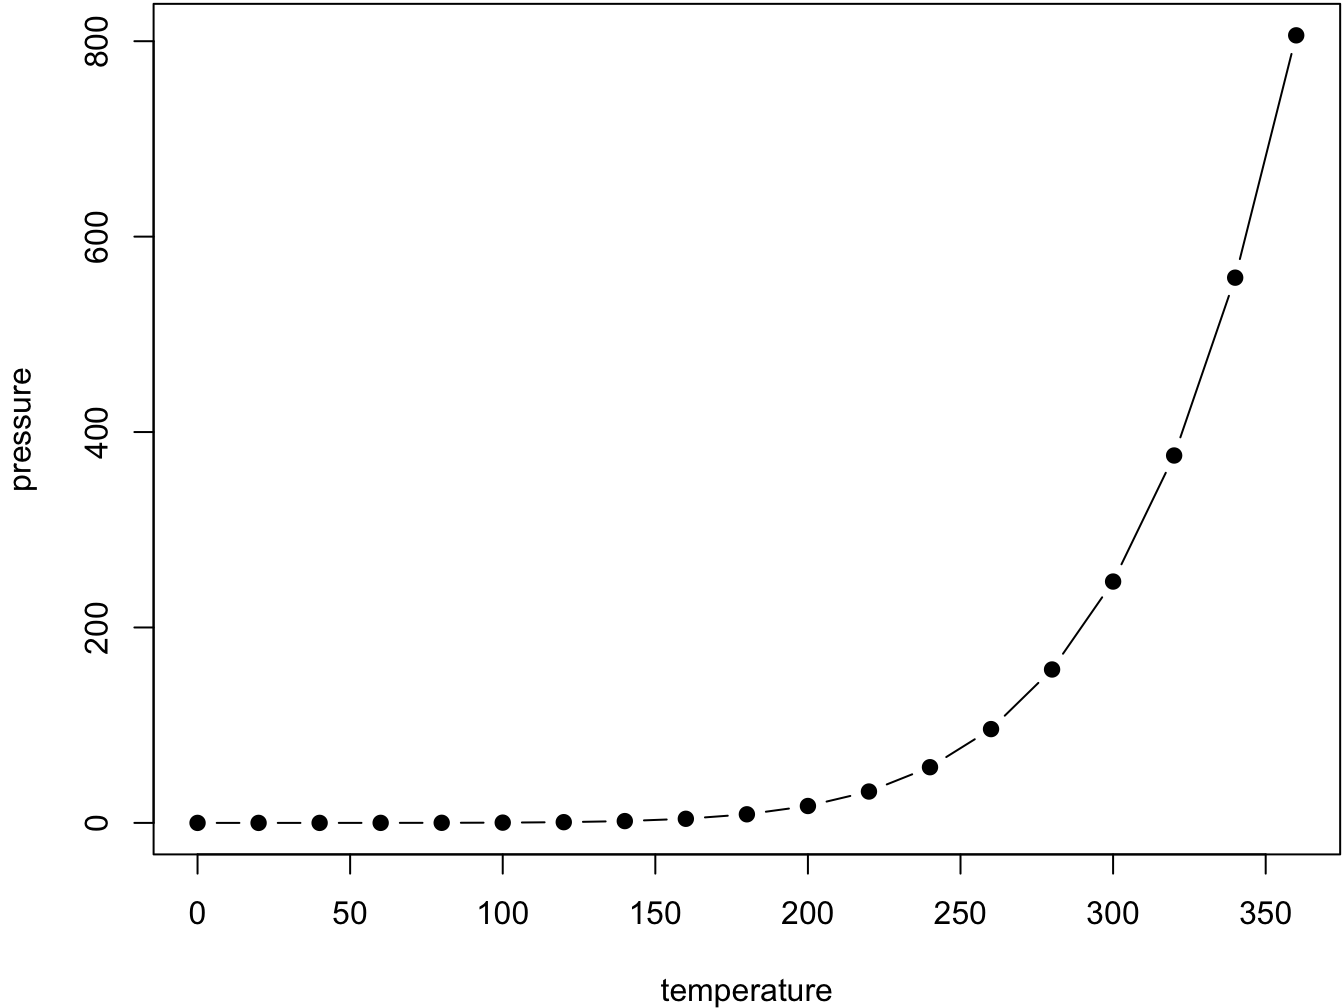
\includegraphics[width=0.8\linewidth]{QuantLife_files/figure-latex/nice-fig-1} 

}

\caption{Here is a nice figure!}\label{fig:nice-fig}
\end{figure}

Reference a figure by its code chunk label with the \texttt{fig:} prefix, e.g., see Figure \ref{fig:nice-fig}. Similarly, you can reference tables generated from \texttt{knitr::kable()}, e.g., see Table \ref{tab:nice-tab}.

\begin{Shaded}
\begin{Highlighting}[]
\NormalTok{knitr}\OperatorTok{::}\KeywordTok{kable}\NormalTok{(}
  \KeywordTok{head}\NormalTok{(iris, }\DecValTok{20}\NormalTok{), }\DataTypeTok{caption =} \StringTok{\textquotesingle{}Here is a nice table!\textquotesingle{}}\NormalTok{,}
  \DataTypeTok{booktabs =} \OtherTok{TRUE}
\NormalTok{)}
\end{Highlighting}
\end{Shaded}

\begin{table}

\caption{\label{tab:nice-tab}Here is a nice table!}
\centering
\begin{tabular}[t]{rrrrl}
\toprule
Sepal.Length & Sepal.Width & Petal.Length & Petal.Width & Species\\
\midrule
5.1 & 3.5 & 1.4 & 0.2 & setosa\\
4.9 & 3.0 & 1.4 & 0.2 & setosa\\
4.7 & 3.2 & 1.3 & 0.2 & setosa\\
4.6 & 3.1 & 1.5 & 0.2 & setosa\\
5.0 & 3.6 & 1.4 & 0.2 & setosa\\
\addlinespace
5.4 & 3.9 & 1.7 & 0.4 & setosa\\
4.6 & 3.4 & 1.4 & 0.3 & setosa\\
5.0 & 3.4 & 1.5 & 0.2 & setosa\\
4.4 & 2.9 & 1.4 & 0.2 & setosa\\
4.9 & 3.1 & 1.5 & 0.1 & setosa\\
\addlinespace
5.4 & 3.7 & 1.5 & 0.2 & setosa\\
4.8 & 3.4 & 1.6 & 0.2 & setosa\\
4.8 & 3.0 & 1.4 & 0.1 & setosa\\
4.3 & 3.0 & 1.1 & 0.1 & setosa\\
5.8 & 4.0 & 1.2 & 0.2 & setosa\\
\addlinespace
5.7 & 4.4 & 1.5 & 0.4 & setosa\\
5.4 & 3.9 & 1.3 & 0.4 & setosa\\
5.1 & 3.5 & 1.4 & 0.3 & setosa\\
5.7 & 3.8 & 1.7 & 0.3 & setosa\\
5.1 & 3.8 & 1.5 & 0.3 & setosa\\
\bottomrule
\end{tabular}
\end{table}

You can write citations, too. For example, we are using the \textbf{bookdown} package \citep{R-bookdown} in this sample book, which was built on top of R Markdown and \textbf{knitr} \citep{xie2015}.

  \bibliography{book.bib,packages.bib}

\end{document}
